%\ihead{\headmark}
\chapter{Signal Processing and Feature Extraction}

Wireless sensor devices and contact-less sensor devices are the current trends in the health informatics. The recent improvements in the sensor devices made it possible for the people to bring this idea
into reality. When medical sensor devices are combined with cloud computing, it can be thought of as a complete
solution for a healthcare system which can be used not only
in hospitals but also can be utilized out of the hospital.
These sensors can monitor some vital signs such as body temperature, respiration, heart rate, blood pressure, ECG or EEG.

\section{Devices}

Multiple non-contact sensors are used to implement a system for this thesis, which collects data of the user and processes them in real-time. The following devices are used in this work:

\subsection{Magnetic Induction Sensor}

The magnetic induction (MI) sensor uses the magnetic fields to measures the small changes in electrical resistance of the thorax. A magnetic coil is used which induces eddy currents within the thorax. This eddy current reinduces a secondary magnetic field which can be measured with the same or another coil. The amplitude of the eddy current is directly proportional to the magnetic flux density and the conduction of the material. Based on this concept, the thorax conductivity, which changes according to the inflation and deflation of the lungs, enable us to capture the breathing of the patient \cite{1742-6596-434-1-012085}. 
\begin{figure}%
	\centering
	
	\subfigure[]{%
		\label{fig:ex3-e}%
		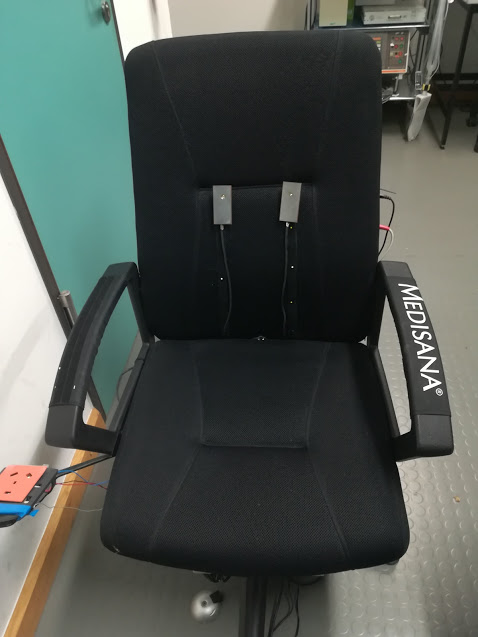
\includegraphics[height=2in]{images/ecg}}%
	\hspace{8pt}%
	\subfigure[][]{%
		\label{fig:ex3-a}%
		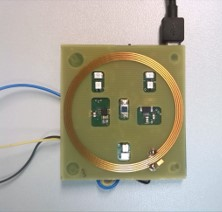
\includegraphics[height=2in]{images/mi}}%
	\hspace{8pt}%
	\subfigure[][]{%
		\label{fig:ex3-b}%
		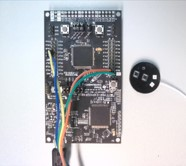
\includegraphics[height=2in]{images/ppg}} \\
	\subfigure[][]{%
		\label{fig:ex3-c}%
		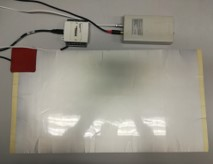
\includegraphics[height=2in]{images/bcg}}%
	\hspace{8pt}%
	\subfigure[][]{%
		\label{fig:ex3-d}%
		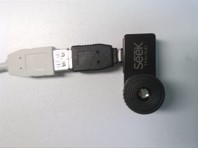
\includegraphics[height=2in]{images/tc}}%
	\caption[A set of sensor devices.]{A set of sensor devices:
		\subref{fig:ex3-e} an ECG sensor;
		\subref{fig:ex3-a} a MI sensor;
		\subref{fig:ex3-b} a PPG sensor;
		\subref{fig:ex3-c} a BCG sensor; and,
		\subref{fig:ex3-d} a thermal camera.}%
	\label{fig:ex3}%
\end{figure}



The MI sensor provides a data packet of 42 bytes, which splits into the attributes shown in Table \ref{tab:att_mi} and the byte identifier is shown in Table \ref{tab:bi_mi}.


As mentioned in Table \ref{tab:bi_mi}, 0x81 and 0x82 represents the byte identifier, but in some cases, it also presents in the data as they are simply the hexadecimal number. The sensor algorithm replaces the data value 0x81 by 0x8101 and 0x82 by 0x8102 in order to differentiate the data values from the byte identifiers. Therefore, to process sensor data correctly, the hexadecimal value 0x8101 should be replaced by 0x81 and 0x8102 by 0x82.

\renewcommand{\arraystretch}{2}
\begin{table}
	\caption{Attributes of MI sensor.} \label{tab:att_mi}
	
	\begin{center}
		\begin{tabular}{ | l | r | }
			\hline
			\textbf{Attributes} & \textbf{Size (Bytes)} \\ \hline
			MI\_RAW  & 4 \\ \hline
			MI  & 4  \\ \hline
			RED\_RAW  & 4  \\ \hline
			ECG\_RAW  & 4  \\ \hline
			IR\_RAW  & 4  \\ \hline
			RED\_AVG  & 4  \\ \hline
			ECG\_AVG  & 4  \\ \hline
			IR\_AVG  & 4  \\ \hline
			ACC\_X  & 2  \\ \hline
			ACC\_Z  & 2  \\ \hline
			ECG\_REF  & 2  \\ \hline
			RESP\_REF  & 2  \\ \hline
			BATTERY  & 2  \\ \hline
		\end{tabular}
	\end{center}
	
\end{table}


\renewcommand{\arraystretch}{2}
\begin{table}
	\caption{Byte identifiers for the MI sensor.} \label{tab:bi_mi}
	
	\begin{center}
		\begin{tabular}{ | l | l | }
			\hline
			\textbf{2-Byte Identifier} & \textbf{Description} \\ \hline
			0x81  & Header \\ \hline
			0x82  & Data Packet  \\ \hline
		\end{tabular}
	\end{center}
	
\end{table}

\subsection{Photoplethysmogram Sensor} \label{sec:ppg_def}
The photoplethysmogram (PPG) sensor is used to measures the variations in blood flow in the body with each heartbeat. It is an optical, simple, low cost and non-invasive technique, which can measure various vital signs at the surface of the skin. A PPG sensor uses a light source to illuminate the skin and a photo-detector to measures the variations in the light intensity associated with changes in the oxygen level in blood. The decrease in light intensity indicates the increase in oxygen level in blood, whereas, increase in light intensity indicates the decrease of oxygen level in blood. They can provide valuable information about the cardiovascular system such as the pulse rate.

The sensor provides PPG signals with 4 different channels, a temperature, and accelerometer coordinates. The size of the data changes according to the attributes, as shown in Table \ref{tab:att_ppg}. The temperature value is sent every one second, while, the frequency rate of PPG channels is 100 samples per second. For the accelerometer coordinates, the data rate is 50 samples per second.

% Please add the following required packages to your document preamble:
% \usepackage{multirow}
\begin{table}[h]
	\centering
	\caption{Attributes of PPG sensor.}
	\label{tab:att_ppg}
	\begin{tabular}{|l|l|r|l|}
		\hline
		\textbf{2-Byte Identifier} & \textbf{Attributes} & \textbf{Size (Bytes)} & \textbf{Data} \\ \hline
		\multirow{4}{*}{} 0x0050 & \multirow{4}{*}{} ppg (8 Bytes) & 2 & Channel 1 \\ \cline{3-4} 
		&                   & 2 & Channel 2 \\ \cline{3-4} 
		&                   & 2 & Channel 3 \\ \cline{3-4} 
		&                   & 2 &  Channel 4 \\ \hline
		0x0054 & Temperature (2 Bytes) & 2 & Temperature \\ \hline
		\multirow{3}{*}{} & \multirow{3}{*}{} & 2 & X Coordinate \\ \cline{3-4} 
		0x0041 & Accelerometer coordinates (6 Bytes) & 2 & Y Coordinate \\ \cline{3-4} 
		&  & 2 & Z Coordinate \\ \hline
	\end{tabular}
\end{table}


\subsection{ECG Sensor}
As described in Section \ref{the_electrocardiogram}, the ECG signal is usually collected by placing electrodes directly on the body but it has several disadvantages as described in Section \ref{electrodes_disadv}. Therefore, non-contact capacitive electrodes have been used to collect the ECG signals. Unlike traditional electrodes, which rely on galvanic contact, the capacitive electrodes are insulated from skin using a dielectric material, such as air gap or clothes \cite{bouchard2017smart}. The ECG signal propagates via skin to the dielectric material and then to the electrodes through a capacitive coupling. The major drawback of this approach is that it is very sensitive to a body motion.

\subsection{Ballistocardiogram Sensor}
The ballistocardiogram (BCG) sensor measures the ballistic forces associated with cardiac contraction and ejection of blood. These ballistic forces are mainly measures by the electromechanical film (EMFi), which converts the mechanical energy into the electrical signal. Most of the time, the EMFi sensing device is placed on a chair or bed, which measures the pressure associated with the cardiac activity.

\subsection{Thermal Camera}
A thermal camera is also used to measures the temperature of the person. A thermal Seek camera captures the thermo temperature images from which the temperature is calculated.

\section{ECG Signal Processing}
The detection of QRS complex is the basis for processing ECG signal. Regardless of what application is required, the accurate detection of QRS complex is a prerequisite for feature extraction. In order to detect the QRS complex accurately, it is necessary to detect the R-peak position correctly. Once the QRS complex is identified, further operations can also be performed on the signal such as heart rate calculation, classification of ECG signal and P and T detection.

The ``QRS Complex'' is the combination of Q, R and S waves and it represents the contraction of the ventricles. It plays a significant role in the detection of cardiac arrhythmias.

Many methods have already been proposed for the detection of QRS complex. These methods fall into 3 categories \cite{5639905}:

\subsection{Filter Method}
The filter method uses a bandpass filter to filter the ECG signal \cite{4122029}\cite{554762}. In this method, a QRS complex is intensified by suppressing the P and T wave. This method is generally very quick and takes less time to implement. But the major drawback of this method is that the frequency band of QRS complex and of noise overlapping affect its performance.

\subsection{Artificial Intelligence Method}
The detection of QRS complex using this method is fast, accurate and more robust, but in reality, it is time-consuming and difficult to implement \cite{126604}\cite{PIETKA1991139}\cite{58593}. Therefore, this method is not very popular and not widely used as compared to the other methods.

\subsection{Wavelet Transform Method}
Wavelet transform method becomes popular in detecting the QRS complex. It is based on time-frequency analysis. It is efficient and takes less to implement. Many researchers have already used wavelet transform for detecting the QRS complex. Yazhu Qiu \cite{PMID:17228741} used Mexican-hat wavelet to detect ECG signal. In the proposed method, although the processing was fast, it sometimes did not detect the onset and offset of QRS complex accurately. Nevertheless, it is considered as faster and easier to implement and it is used to extract the ECG signal features in this thesis.


\section{Wavelet Transform}

A wavelet transform is a very useful tool for analyzing the signal simultaneously in both time and frequency domain \cite{addison2017illustrated}. It uses a little wavelike functions known as \textbf{\textit{wavelets}}. Wavelets are used to transform a signal into another representation where signal information can be viewed in a more useful form.

Generally, there are two operations involved with wavelet. Either they can be stretched or squeezed or can be translated to other locations on the signal and if the wavelet matches the shape of the signal at specific location or scale, it produces a large transform value. And similarly, if the signal and the wavelet do not correlate, it produces a low transformed value. There is a single function called ``mother wavelet'' which is stretched or translated to produce a family of basis functions known as ``daughter wavelet''. A mother wavelet is defined as:

\begin{equation} \label{eqn_mother_wavelet}
{\Psi_{a,b}(t) = \frac{1}{\sqrt{|a|}}\Psi \bigg(\frac{t-b}{a}\bigg),\quad a, b \in \mathbb{R}, a \neq 0}
\end{equation}

where \textit{a} is the scaling parameter which measures the degree of the scale, and \textit{b} is the translation parameter, which measures the time location of the wavelet. If |\textit{a}| < 1, then it mainly corresponds to higher frequencies. And on the other hand, if |\textit{a}| > 1, it corresponds to lower frequencies. It is important to note here that the variation in time and frequency scale of the wavelet is supervised by the Heisenberg's uncertainty principle. At large scale, the time domain is not very clear, whereas, in the frequency domain is much finer. As the scale decreases, the frequency domain becomes worse, whereas, time domain becomes finer.

The wavelet transform of a signal $f(x)$ is defined as:

\begin{equation} \label{eqn_wavelet_transform}
{X_{W}(a, b) = \frac{1}{\sqrt{|a|}} \int_{-\infty}^\infty \bigg(\frac{t-b}{a}\bigg)f(x) \mathrm{d}x}
\end{equation}

If $a=2^j (j \in Z)$, then the wavelet transform is called the dyadic wavelet transform or the binary wavelet transform \cite{119727}. 
To calculate the dyadic wavelet transform of a signal, a mother wavelet is first chosen and then dilated by a power of two. The Quadratic Spline wavelet is used with ECG signal as the mother wavelet. It has a property that the sharp edges occur at the zero crossing point in the transformation, which corresponds to the local maxima or minima of the smoothed signal. The dyadic wavelet transform of a signal $f(n)$ can be calculated by using Mallat's Algorithm \cite{5639905}. 

\section{Mallat's Algorithm}
Mallat algorithm \cite{119727} for the signal $f(n)$ is defined as follows:

\begin{equation} 
{ s_{2^j}f(n) = \sum h_ks_{2^{j-1}}f(n - 2^{j-1}k),   }
\end{equation}

\begin{equation} 
{ w_{2^j}f(n) = \sum g_ks_{2^{j-1}}f(n - 2^{j-1}k).   }
\end{equation}

where, $s_{2^0}f(n)$ is the original signal to be processed, in this case, it is the ECG signal. $w_{2^j}f(n)$ is the wavelet transform of the input signal $f(n)$ at scale $2^j$. $h_k$ and $g_k$ are the coefficients of a low-pass filter and high-pass filter respectively. The wavelet transform of a signal $f(n)$ is obtained by passing the input signal through a digital filter bank, which consists of a low-pass and high-pass filters. The design and implementation of the Wavelet transform is based on perfect reconstruction filter banks. The coefficients of low-pass filter $H(z)$ and high-pass filter $G(z)$ can be calculated by constructing a filter bank.

\section{Filter Bank Construction}
A biorthogonal filter bank is designed based on Quadratic Spline wavelet. A filter bank is a set of filters and sampling operators \cite{strang1996wavelets}. The downsampling operators are decimators, whereas, upsampling operators are expanders. In a 2-channel filter bank, the analysis and synthesis phase both contain a low-pass and a high-pass filter. These filters are ${H_{0}(z)}$ and ${H_{1}(z)}$ for the analysis phase, and ${G_{0}(z)}$ and ${G_{1}(z)}$ for the synthesis phase respectively \cite{wang2001using}, as shown in Figure \ref{fig:2_channel_filter_bank}. After passing the input signal $X[n]$ from the filters, the resulting signal is first down-sampled by 2 and then up-sampled by 2 respectively, producing the final output signal $Y[n]$. 

The filters ${H_{0}(z)}$ and ${H_{1}(z)}$ are not ideal filters, therefore, their responses overlap, there is aliasing in each channel and there is distortion. The synthesis filters ${G_{0}(z)}$ and ${G_{1}(z)}$ should be adjusted according to the analysis filters ${H_{0}(z)}$ and ${H_{1}(z)}$ to cancel out the error.

%\begin{figure}[h] for figure at the place, where we put the picture.
\begin{figure}[h]
	\centering
	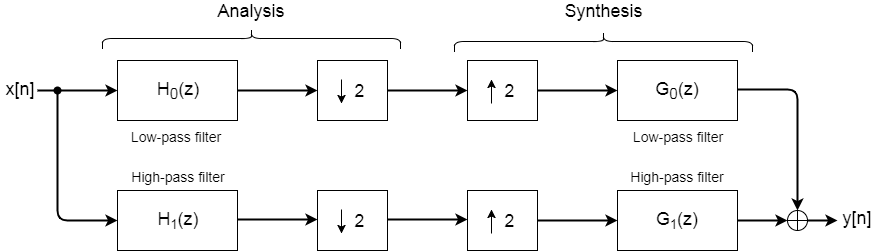
\includegraphics[width=160mm]{images/2_channel_filter_bank}
	\caption{Two-channel filter bank}
	\label{fig:2_channel_filter_bank}
\end{figure}



The idea is to determine $H_0$, $H_1$, $G_0$ and $G_1$ such that, $Y[n]$ is a delayed version of input signal $X[n]$. This is called as perfect reconstruction filter bank. A perfect reconstruction filter bank is also known as ``biorthogonal'' and the associated filters as biorthogonal filters. A perfect reconstruction with an $l-$step delayed in $z$ domain without upsampling and downsampling represented as:


\begin{equation} \label{eqn:basic_tr}
{H_{0}(z)G_{0}(z) + H_{1}(z)G_{1}(z) = z^{-l}}
\end{equation}


The combination of downsampler ($\downarrow$ 2) and an upsampler ($\uparrow$ 2) removes the odd number components. In $z$ domain, it can be written as:

\begin{equation} \label{eqn_wavelet_transform}
{(\downarrow 2)(\uparrow 2)H_{0}X = \frac{1}{2}[H_{0}(z)X(z) + H_{0}(-z)X(-z)]}
\end{equation}

It contains only the even components as the odd components have already been removed. The term $H_{0}(-z)X(-z)$ is an aliasing term. This aliasing term has to cancel the aliasing effect from the other channel to remove the alias.


After passing the input signal from the channel 1, it produces:

\begin{equation} \label{eqn_wavelet_transform}
{Y_{0}(z) = \frac{1}{2}G_{0}(z)[H_{0}(z)X(z) + H_{0}(-z)X(-z)]}
\end{equation}

Similarly, for the 2nd channel, it produces:


\begin{equation} \label{eqn_wavelet_transform}
{Y_{1}(z) = \frac{1}{2}G_{1}(z)[H_{1}(z)X(z) + H_{1}(-z)X(-z)]}
\end{equation}

Adding the output of these 2 channels produce the final output.



\begin{equation} \label{eq1}
\begin{split}
Y(z)  &= Y_{0}(z) + Y_{1}(z) \\
&= \frac{1}{2}G_{0}(z)[H_{0}(z)X(z) + H_{0}(-z)X(-z)] + \frac{1}{2}G_{1}(z)[H_{1}(z)X(z) + H_{1}(-z)X(-z)]
\end{split}
\end{equation}


Arranging $Y(z)$ in such a way so that, one part depends on $X(z)$ and the other part on $X(-z)$. We get,

\begin{equation} \label{eqn:cmp}
{Y(z) = \frac{1}{2}[G_{0}(z)H_{0}(z) + G_{1}(z)H_{1}(z)]X(z) + \frac{1}{2}[G_{0}(z)H_{0}(-z) + G_{1}(z)H_{1}(-z)]X(-z)}
\end{equation}

In Equation \ref{eqn:cmp}, the part that depends on $X(-z)$ is the aliasing part, and the part that depends on $X(z)$ is the distortion part.

%In order to satisfy the condition, $Y(n) = X(n-k)$ ($Y(z) = X(z)z^{-k}$) i.e., %the output signal $Y(z)$ to be some sort of delayed version of input signal, we %need to satisfy 2 conditions:


The perfect reconstruction for filter bank can be achieved if the following two conditions are satisfied.

\begin{enumerate}
	\item No aliasing: 
	\begin{equation} \label{eqn:noalias}
	{G_{0}(z)H_{0}(-z) + G_{1}(z)H_{1}(-z) = 0}
	\end{equation}
	\item No distortion:
	\begin{equation} \label{eqn:nodistor}
	{G_{0}(z)H_{0}(z) + G_{1}(z)H_{1}(z) = mz^{-k}}
	\end{equation}
\end{enumerate}


where $m$ is a constant and $k$ is a time delay.

In order to satisfy condition 1 i.e., to get rid of aliasing, choose:

\begin{align}
	\label{eqn:antialiasing_values}
	\begin{split}
		G_0(z) &=  H_1(-z), \\ 
		G_1(z) &=  -H_0(-z)
	\end{split}
\end{align}

Substituting the values of Equation \ref{eqn:antialiasing_values} in  \ref{eqn:noalias} yields:

\begin{equation} \label{eqn:aliasrem}
{H_{0}(-z)H_1(-z)-H_0(-z)H_{1}(-z) = 0}
\end{equation}

which implies to 0, hence the aliasing is removed.

In order to remove the distortion, i.e, to satisfy equation \ref{eqn:nodistor}, lets assume that,

\begin{equation}\label{eqn:p0} 
{P_0(z)=G_{0}(z)H_{0}(z)}
\end{equation}

This is a low-pass product filter. The high-pass product filer is ${P_1(z)=G_{1}(z)H_{1}(z)}$. The relationship between the terms $P_0$ and $P_1$ can be deduce by Equation \ref{eqn:antialiasing_values}:

\begin{equation} 
{P_1(z) = G_{1}(z)H_{1}(z) = -H_{0}(-z)G_{0}(-z) = -P_0(-z)}
\end{equation}

The equation \ref{eqn:nodistor} can be re-written as:

\begin{equation}\label{eqn:updated_no_dist} 
{P_0(z) - P_0(-z) =  mz^{-k}}
\end{equation}

The design of 2-channel filter bank is now reduced to only two steps:

\begin{enumerate}
	\item Design a low-pass filter which satisfy Equation \ref{eqn:updated_no_dist}.
	\item Factorize $P_0$ to find the values of $H_0$ and $G_0$.
\end{enumerate}

Equation \ref{eqn:updated_no_dist} can be further simplified by normalizing $P_0(z)$ by $z^k$ to center it. Substituting $P(z)$ by $z^kP_0(z)$ and $P(-z)$ by $-z^kP_0(-z)$ produces:


\begin{equation}\label{eqn:piern} 
{P(z) + P(-z) =  m}
\end{equation}

Equation \ref{eqn:piern} implies that $P(Z)$ is a half-band filter, in which all even powers of $z$ in $P(z)$ are zero except for the constant term (coefficient of the term $z^0$). Furthermore, all the odd powers cancel out when $P(z)$ and $P(-z)$ are added. 


One possibility to design the low-pass filter $P_0(z)$ is to use the Daubechies construction \cite{strang1996wavelets}:

\begin{equation}\label{eqn:daubechies} 
{P_0(z) = (1 + z^{-1})^{2p}Q(z)}
\end{equation}

$P_0(z)$ is called ``maxflat filter'' where $p$ can be any integer and has $2p$ coefficients, i.e., the length of the filter. $(1 + z^{-1})^{2p}$ is called \textit{binomial filter} and it is a spline filter, and $Q(z)$ be a polynomial of degree $(2p-2)$ is chosen such that $P_0(z)$ satisfy  the half-band filter property. Moreover, the order of $P_0(z)$ is always an even number. $p$ defines the number of zeros to be placed at $\pi$ in a unit circle. 
%The filter bank is orthogonal and the product filters $P_0(z)$ and %$P_1(z)$ have a length of $4p-2$. 

Any value of $p$ can be chosen and the polynomial $Q(z)$ depends on the value of $p$, i.e., $Q(z)$ should be chosen in such a way that it satisfies the half-band filter property. If $p=1$, then this represents the Haar case and it has 2 coefficients.

In this case, $p=2$ is chosen. Therefore, the number of coefficients are 4 and degree of $Q(z)$ be 2. Then Equation \ref{eqn:daubechies} becomes:

\begin{equation}\label{eqn:daubechies_upd} 
{P_0(z) = (1 + z^{-1})^{4}Q(z)}
\end{equation}

Let $Q(z)$ be of form,

\begin{equation}\label{eqn:qz} 
{Q(z) = a+bz^{-1}+az^{-2}}
\end{equation}


Substituting Equation \ref{eqn:qz} in \ref{eqn:daubechies_upd} produces:

\begin{equation}\label{eqn:producer} 
{P_0(z) = a + (4a+b)z^{-1} + (7a + 4b)z^{-2} + (8a+6b)z^{-3} + (7a+4b)z^{-4} + (4a+b)z^{-5} + az^{-6}}
\end{equation}

To satisfy the condition on $P_0(z)$, equating all the coefficients of odd power of $z$ to 0, except for the center term, i.e., term at $z^{-3}$ which equates to 1, produces:

\begin{equation}\label{eqn:yiedl} 
{4a + b = 0}
\end{equation}


\begin{equation}\label{eqn:yied2} 
{8a + 6b = 1}
\end{equation}

Solving Equation \ref{eqn:yiedl} and \ref{eqn:yied2} yields:

\begin{equation}\label{eqn:values} 
{a = \frac{-1}{16}, b=\frac{1}{4}}
\end{equation}


From Equation \ref{eqn:daubechies_upd}, \ref{eqn:qz} and \ref{eqn:values}, we get:

\begin{equation} 
{P_0(z) = \frac{(1 + z^{-1})^4(-1 + 4z^{-1} - z^{-2})}{16}}
\end{equation}

Factorizing $P_0(z)$ to get $H_0(z)$ and $G_0(z)$:

\begin{equation} \label{eq1}
\begin{split}
H_0(z) & = \frac{(1 + z^{-1})^3}{4} \\
& = \frac{(1 + 3z^{-1} + 3z^{-2} + z^{-3})}{4}
\end{split}
\end{equation}


%and


\begin{equation} \label{eq1}
\begin{split}
G_0(z) & = \frac{(1 + z^{-1})(-1 + 4z^{-1} - z^{-2})}{4} \\
& = \frac{(-1 + 3z^{-1} + 3z^{-2} - z^{-3})}{4}
\end{split}
\end{equation}


Then by equation \ref{eqn:antialiasing_values}, we have:


\begin{equation} \label{eq1}
\begin{split}
H_1(z) = G_0(-z) \\
& = \frac{(-1 - 3z^{-1} + 3z^{-2} + z^{-3})}{4}
\end{split}
\end{equation}

%and

\begin{equation} \label{eq1}
\begin{split}
G_1(z) = -H_0(-z) \\
& = \frac{(-1 + 3z^{-1} - 3z^{-2} + z^{-3})}{4}
\end{split}
\end{equation}

Therefore, the filter coefficients are:

\begin{equation}
\label{eqn:filters}
\begin{aligned}
h_0(0) & =  \quad \frac{1}{4}    & \quad &\quad  h_0(1) &= \quad \frac{3}{4} \\
h_0(2) & =  \quad \frac{3}{4}    & \quad &\quad   h_0(3) &= \quad \frac{1}{4} \\[1ex]
h_1(0) & =  \quad \frac{- 1}{4}  & \quad &\quad   h_1(1) &= \quad \frac{-3}{4} \\
h_1(2) & =  \quad \frac{3}{4}    & \quad &\quad   h_1(3) &= \quad \frac{1}{4} \\[1ex]
g_0(0) & =  \quad \frac{-1}{4}   & \quad &\quad   g_0(1) &= \quad \frac{3}{4} \\
g_0(2) & =  \quad \frac{3}{4}    & \quad &\quad   g_0(3) &= \quad \frac{-1}{4} \\[1ex]
g_1(0) & =  \quad \frac{-1}{4}   & \quad &\quad   g_1(1) &= \quad \frac{3}{4} \\
g_1(2) & =  \quad \frac{-3}{4}   & \quad &\quad   g_1(3) &= \quad \frac{1}{4}
\end{aligned}
\end{equation}

The coefficients of filters are just simple fractions, therefore, the amount of computation and time needed for the transformation is small. As our interest is only in the decomposition of the signal, therefore, we will consider only the $H_0$ and $H_1$ filters coefficients.

Let $f(n)$ be the ECG signal, then the wavelet transform of $f(n)$ can be calculated by using Mallat algorithm as follows:

\begin{equation} 
{ s_{2^0}f(n) = f(n)   }
\end{equation}

\begin{equation} \label{eqn:approx}
{ s_{2^j}f(n) = \frac{1}{4}s_{2^{j-1}}f(n) + \frac{3}{4}s_{2^{j-1}}f(n-2^{j-1}) + \frac{3}{4}s_{2^{j-1}}f(n-2^{j}) + \frac{1}{4}s_{2^{j-1}}f(n-2^{j} * 3) }
\end{equation}

\begin{equation} \label{eqn:detail}
{ w_{2^j}f(n) = \frac{-1}{4}s_{2^{j-1}}f(n) + \frac{-3}{4}s_{2^{j-1}}f(n-2^{j-1}) + \frac{3}{4}s_{2^{j-1}}f(n-2^{j}) + \frac{1}{4}s_{2^{j-1}}f(n-2^{j} * 3) }
\end{equation}

where $w_{2^j}f(n)$ is the Biorthogonal Spline Wavelet Transform of ECG signal at scale $2^j$.


\section{Dataset}

The MIT-BIH Arrhythmia dataset is used for the implementation of the system. It contains 48 hours of recording of 47 subjects. Each record contains 2 signals, namely MLII and V5, with a recording of 30 minutes duration. The sample rate for the recording is 360 samples per second per channel with 11-bit resolution over a 10mV range. Each record consists of 3 files:

\begin{itemize}
	\item Header file (.hea): It contains information such as the number of samples, sampling frequency, ECG signal format, number of ECG leads and their types, patient's history and the detailed clinical information.
	
	\item ECG signals (.dat): It contains the original signal values of both MLII and V5 leads. The signals from MLII lead are used in the analysis.
	
	\item Attribute file (.atr): It contains the annotation information of the ECG signal, annotated by the doctors.
\end{itemize}


\begin{figure}[h]
	\centering
	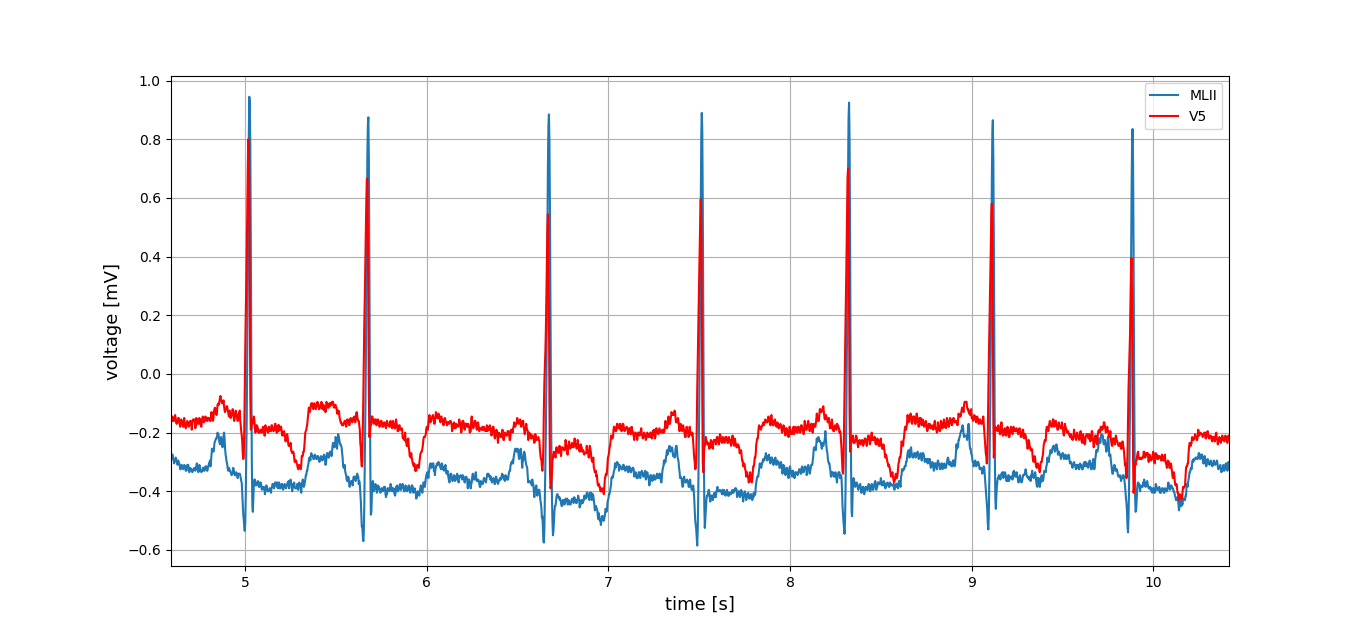
\includegraphics[width=15cm,height=12cm,keepaspectratio=true]{images/all_signals}
	\caption{
		The ECG signals from MIT-BIH dataset.
	}
	\label{fig:all_signals}
\end{figure}

There is a specific python package \textit{wfdb-python} available for reading the data from the MIT-BIH dataset. The ECG signals of one of the patients can be seen in Figure \ref{fig:all_signals}. It contains 2 signals, namely, MLII and V5.




The signals are generally contaminated with noise or baseline drift. Therefore, they are required to be processed in order to achieve better signals.


\section{Preprocessing}
Two different methods have been used to remove the noise and artifacts from the signal in the system implementation.

\begin{enumerate}
	\item Wavelet transform method
	\item Band-pass filter method
\end{enumerate}

\subsection{Wavelet Transform Method}

The wavelet transform decomposes the signal into different frequency bands by passing the signal through high-pass and low-pass filter respectively, which results in 2 sets of coefficients namely, approximation coefficients and detail coefficients. The approximation coefficients contain the low-pass filter coefficients and the detail coefficients contain the high-pass filter coefficients. The next step is to split the approximation coefficients again into 2 parts using the same procedure and so on.

\begin{figure}[h]
	\centering
	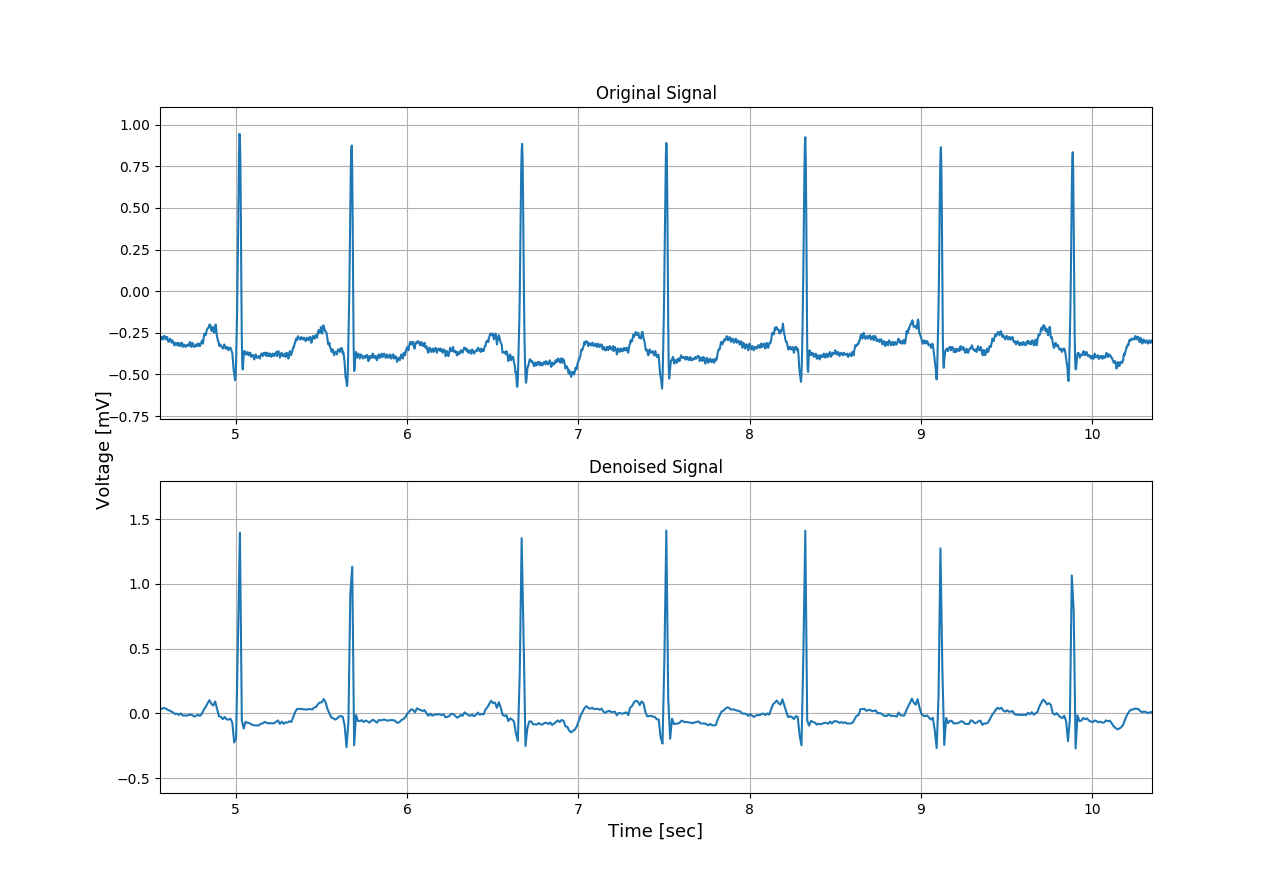
\includegraphics[width=15cm,height=12cm,keepaspectratio=true]{images/wavelet_denoised_1}
	\caption{
		The filtered ECG signal using wavelet.
	}
	\label{fig:wavelet_denoised}
\end{figure}


The original signal contains the high-frequency noise and the baseline drift. The wavelet transform can be used to remove the corresponding noises and the baseline drift. The process starts by decomposing the original signal into 8 layers using Wavelet type \textit{bior2.6}, which results in the corresponding detail and approximation coefficients. Mostly, the layers 1 and 2 of the detail coefficients contain the high-frequency noise and the layer 8 of the approximation coefficients contain the baseline drift. Therefore, the layers 1 and 2 of the detail coefficients and layer 8 of the approximation coefficients are set to 0, which then results in the de-noised signal with no baseline drift. The resulting ECG signal is shown in Figure \ref{fig:wavelet_denoised}. 




\subsection{Band-pass Filter Method}
A band-pass filter is a type of filter, which passes frequencies only in a certain range or spread without disturbing the input signal. A band-pass filter can be used to reduce the baseline drift, motion artifacts and high-frequency noise from the ECG signal. A passband of 0.5 Hz to 40 Hz has been used. After applying the band-pass filter, this results in the denoised signal with no high-frequency and baseline drift. The denoised signal is shown in Figure \ref{fig:bandpass_denoised}. 

\begin{figure}[h]
	\centering
	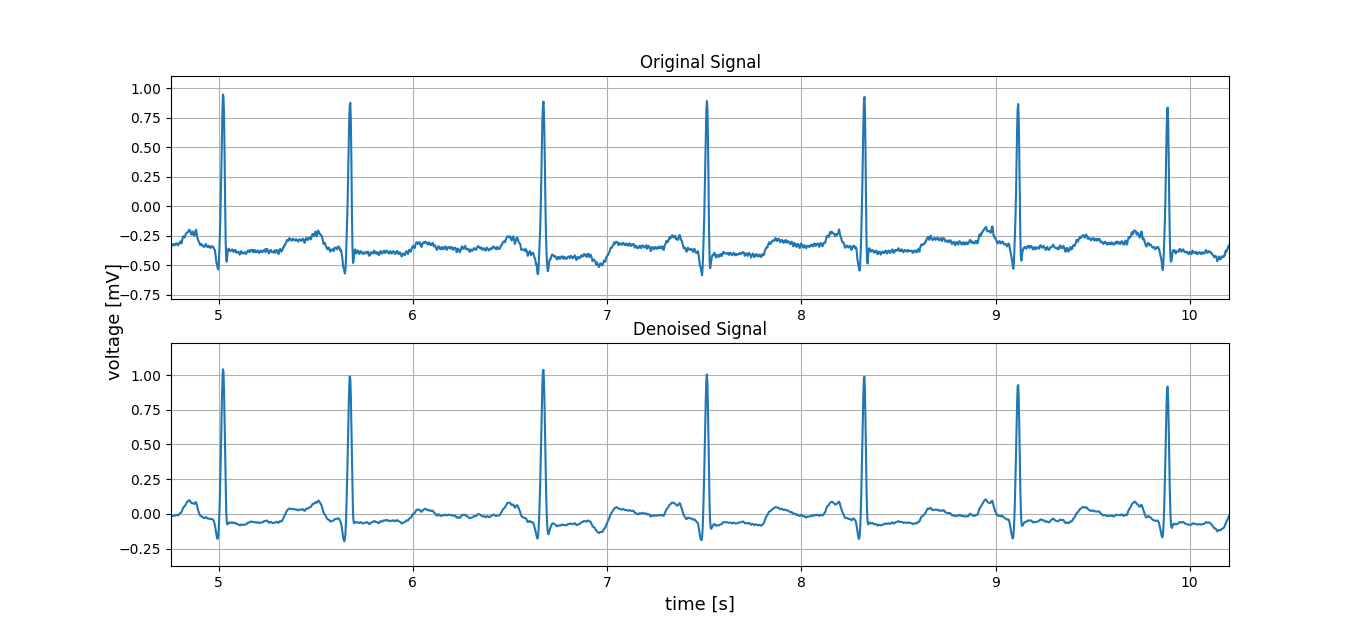
\includegraphics[width=15cm,height=12cm,keepaspectratio=true]{images/bandpass_denoised_1}
	\caption{
		The filtered ECG signal using bandpass filter.
	}
	\label{fig:bandpass_denoised}
\end{figure}


\section{QRS Detection}\label{sec:ecg_det}

From Equation \ref{eqn:approx} and \ref{eqn:detail}, the Biorthogonal Spline Wavelet Transform of ECG signal is obtained, which is the first derivative of the signal at different scales. The signal is decomposed into 4 levels, as shown in  Figure ~\ref{fig:detail_coefficients}. The procedure starts by first locating the R peaks and then the onset and offset of QRS complexes, and finally the onset and offset of P and T waves. Due to Wavelet characteristic derivative, this wavelet transforms the signal maxima and minima into the zero crossing point at the different scales, which makes it easier to detect the location of P, QRS and T waves \cite{e2010cardiac}.


\begin{figure}[htpb]
	\centering
	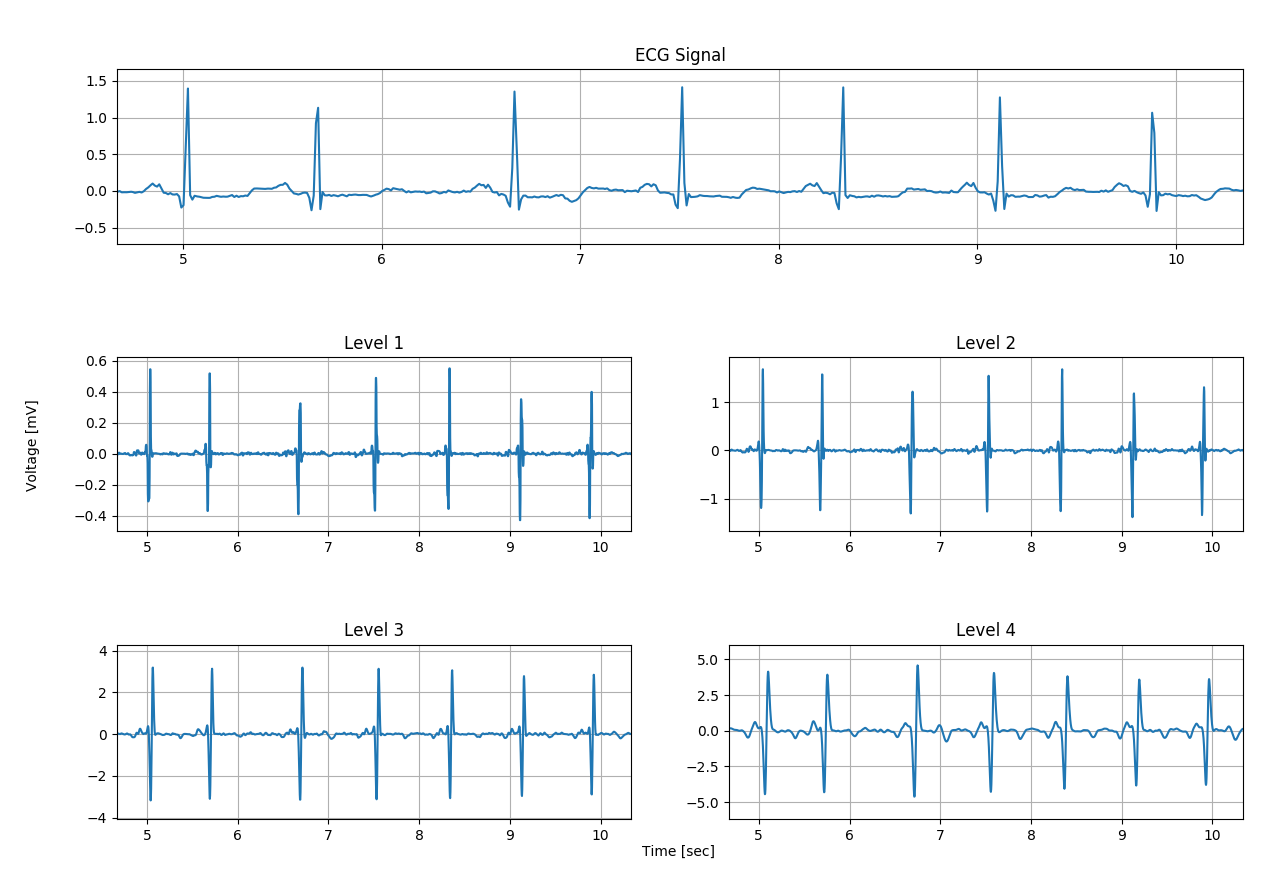
\includegraphics[width=14cm,height=17cm,keepaspectratio=true]{images/detail_coefficients}
	\caption{
		ECG signal and its decomposition at different scales.
	}
	\label{fig:detail_coefficients}
\end{figure}

\renewcommand{\arraystretch}{2}
\begin{table}[h]
	\caption{Wavelet transform ECG signal frequency range\cite{shang2014qrs}.} \label{tab:qrsenergy}
	
	\begin{center}
		\begin{tabular}{ | l | r | }
			\hline
			Transform Scale & Frequency Range (Hz) \\ \hline
			${2^1}$  & 90.0{\raise.17ex\hbox{$\scriptstyle\sim$}}180.0 \\ \hline
			${2^2}$  & 29.92{\raise.17ex\hbox{$\scriptstyle\sim$}}84.24  \\ \hline
			${2^3}$  & 1.52{\raise.17ex\hbox{$\scriptstyle\sim$}}38.88  \\ \hline
			${2^4}$  & 5.76{\raise.17ex\hbox{$\scriptstyle\sim$}}19.44  \\ 
			\hline
		\end{tabular}
	\end{center}
	
\end{table}

Most of the QRS complex energy lies between 3 Hz and 40 Hz, and it corresponds to the $3^{rd}$ scale as shown in Table \ref{tab:qrsenergy}. The R peaks correspond to the zero-crossing point of the modulus maxima pair, with a little delay, therefore, first all the positive and negative extrema on scale 3 be identified. The extrema are shown in Figure \ref{fig:maximas_on_level_3}.  To reduce the influence of noise and other interference in locating the R peaks, the scale 3 signal is divided into four parts, let's say, $A1, A2, A3$ and $A4$. To find the average maximum and minimum values, the maximum and minimum values from each part are identified.


\begin{equation} 
{ MAX = \frac{max(A1) + max(A2) + max(A3) + max(A4)}{4}}
\end{equation}


\begin{equation} 
{ MIN = \frac{min(A1) + min(A2) + min(A3) + min(A4)}{4}}
\end{equation}


Not all the extrema are important, therefore, only modulus maxima pair in certain scope can be focused and the rest can be ignored. The threshold are calculated as:
\begin{equation}  \label{eqn:thresholds}
{ Th_1 = \frac{MAX}{2}} , { Th_2 = \frac{MIN}{2}} 
\end{equation}

The threshold values can be adjusted. If they are too big, then the missing probability of R peaks would be higher and if they are too low, then the noise or interference can be misdetected as R peaks. The thresholds defined above provided the best result in our experiment. The modulus maxima pair are shown in Figure \ref{fig:max_pair}.

\begin{figure}[]
	\centering
	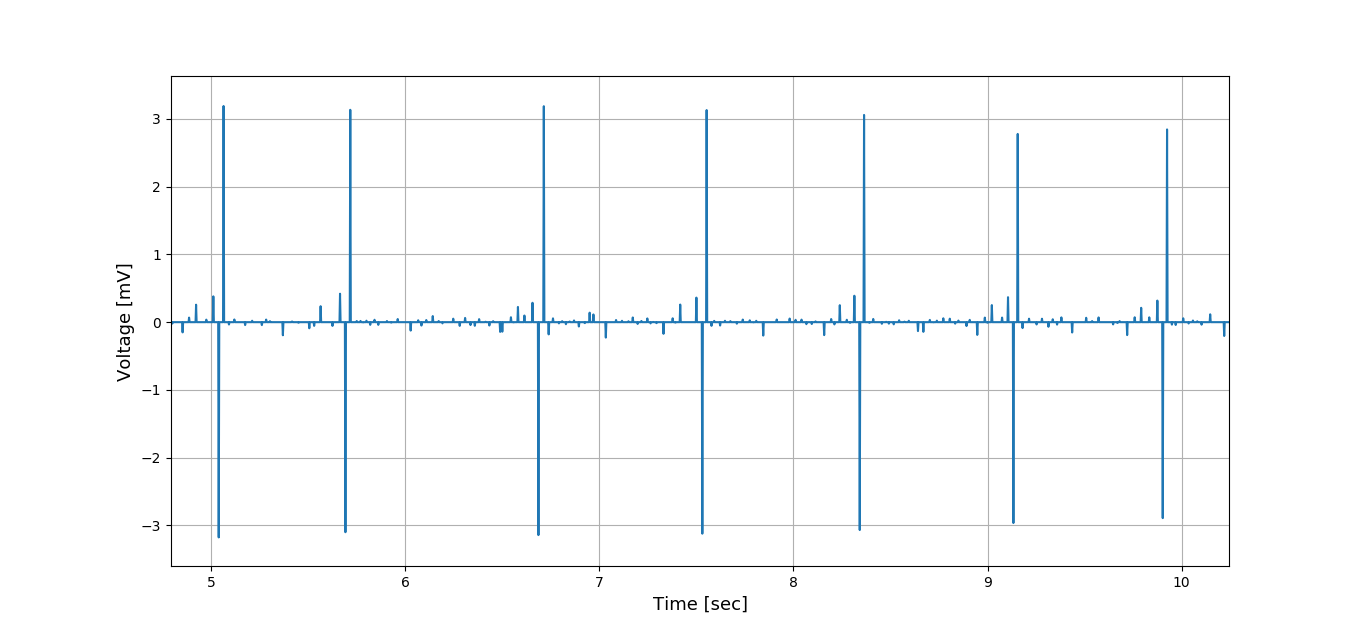
\includegraphics[width=15cm,height=15cm,keepaspectratio=true]{images/maximas_on_level_3}
	\caption{
		Maximum and minimum values on scale 3.
	}
	\label{fig:maximas_on_level_3}
\end{figure}

\begin{figure}[htpb]
	\centering
	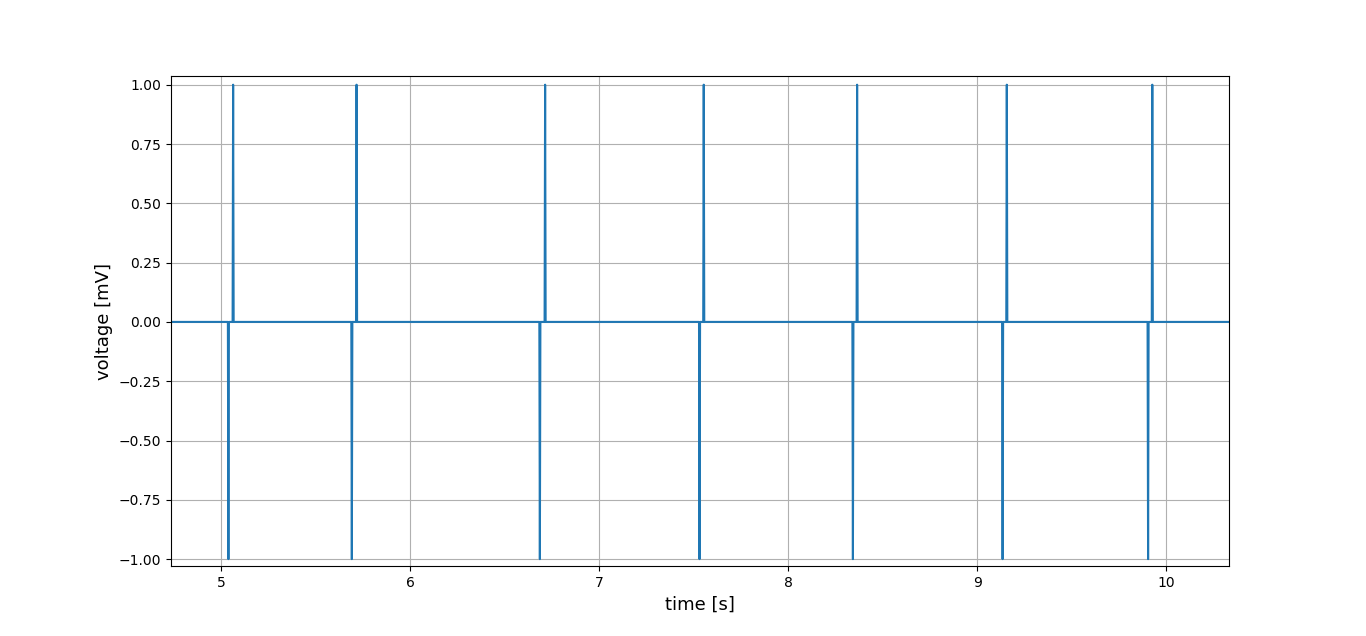
\includegraphics[width=15cm,height=12cm,keepaspectratio=true]{images/max_pair}
	\caption{
		Maximum and minimum values pair for finding the R peaks.
	}
	\label{fig:max_pair}
\end{figure}


The best modulus maxima pair corresponds to the R peaks and the value of R peaks lie at the zero-crossing point of modulus maxima pair with a little delay. For compensating the delay, a maximum value can be searched in the window of 20 points to the zero-crossing point to determine the accurate position of R peaks. 

To compensate the false R peak detection or misdetection, the distance between the adjacent R peaks is calculated. If the distance is less than 40\% of the average RR interval, then one of the peaks is misdetected. Therefore, the larger one is kept as R peak and the smaller one is eliminated.

If the distance between adjacent R peaks is greater than 160\% of the average RR interval, it is considered as misdetection. Therefore, the threshold values defined in Equation \ref{eqn:thresholds}, are further reduced and R peak is searched again in the adjacent R peaks window or interval.


The detected R-peaks are shown in Figure \ref{fig:r_peaks}. The flowchart for finding the R peaks is shown in Figure \ref{fig:r_peaks_flow_chart}.

\begin{figure}[htpb]
	\centering
	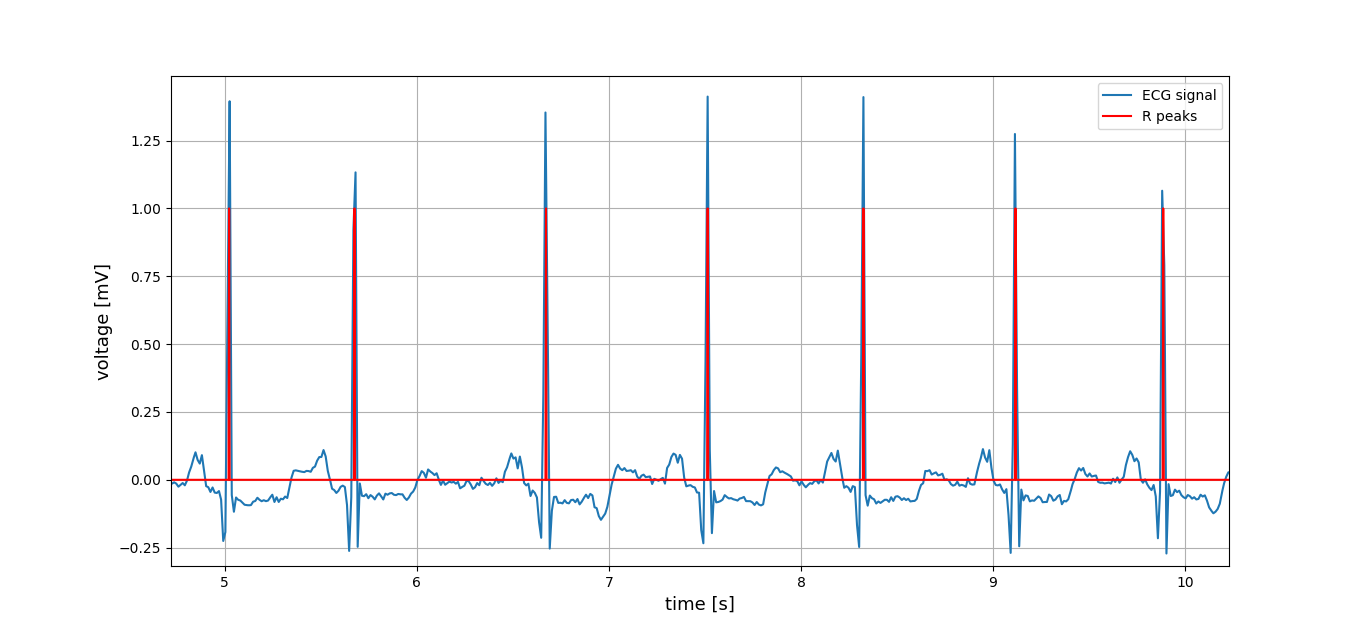
\includegraphics[width=15cm,height=15cm,keepaspectratio=true]{images/r_peaks}
	\caption{
		Detected R peaks.
	}
	\label{fig:r_peaks}
\end{figure}


\begin{figure}[htpb]
	\centering
	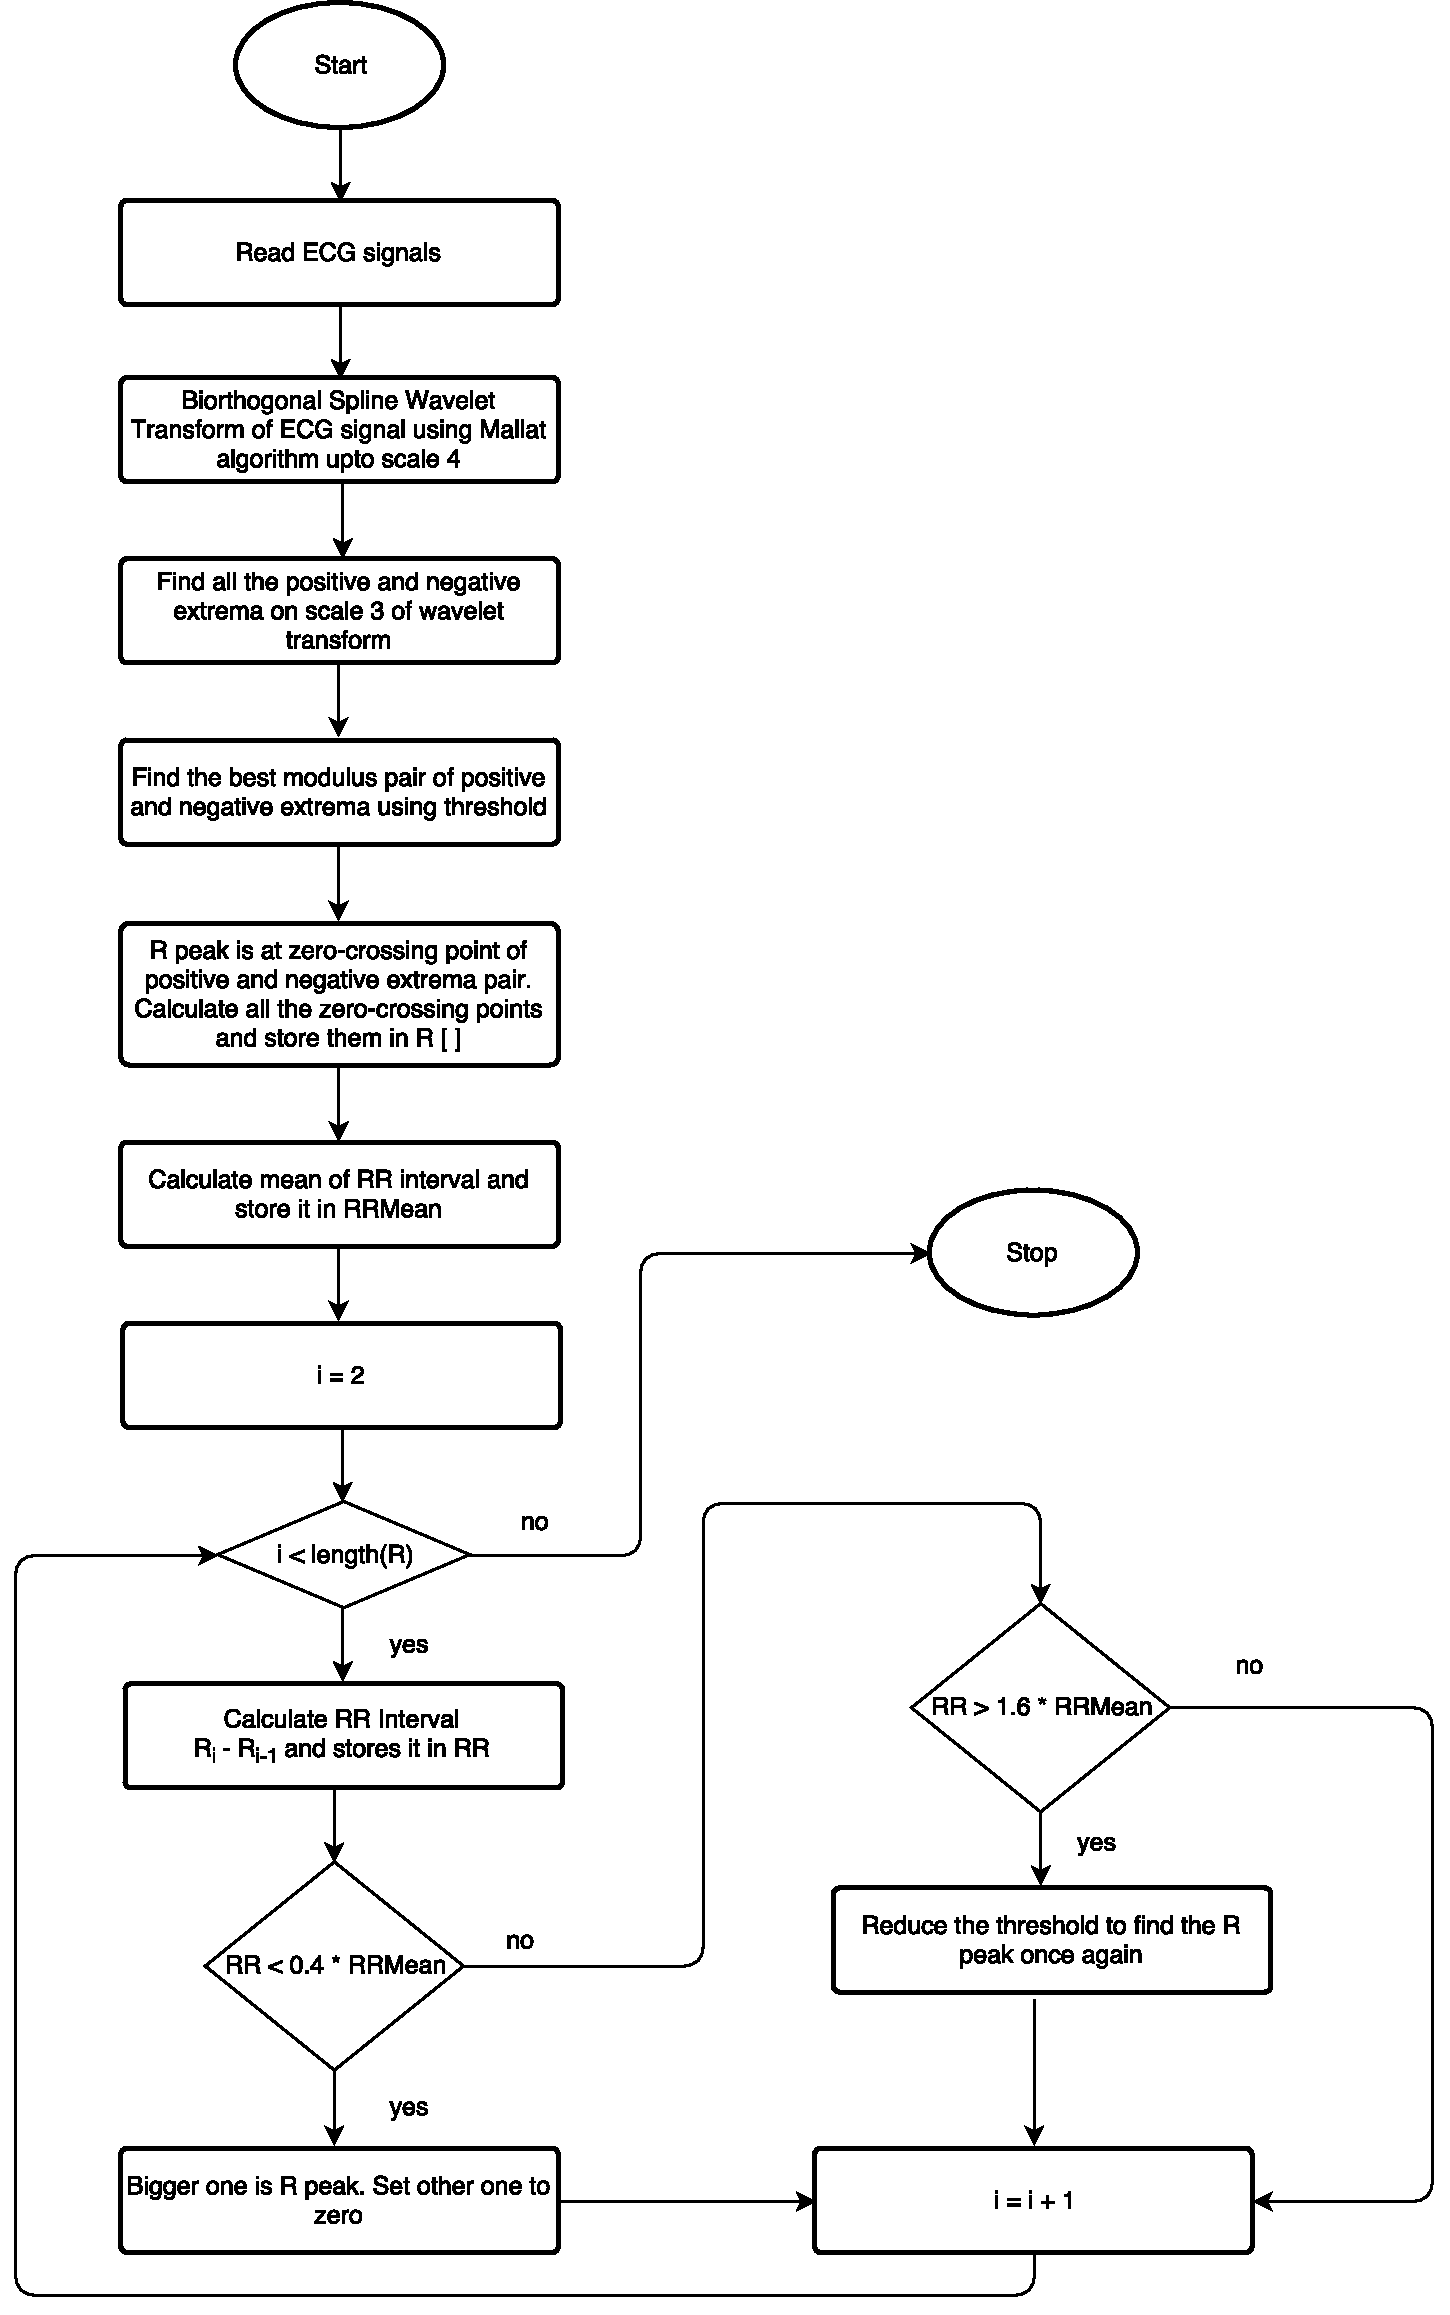
\includegraphics[width=25cm,height=22cm,keepaspectratio=true]{images/qrs.pdf}
	\caption{
		Flowchart for locating R peaks.
	}
	\label{fig:r_peaks_flow_chart}
\end{figure}


\begin{figure}[htpb]
	\centering
	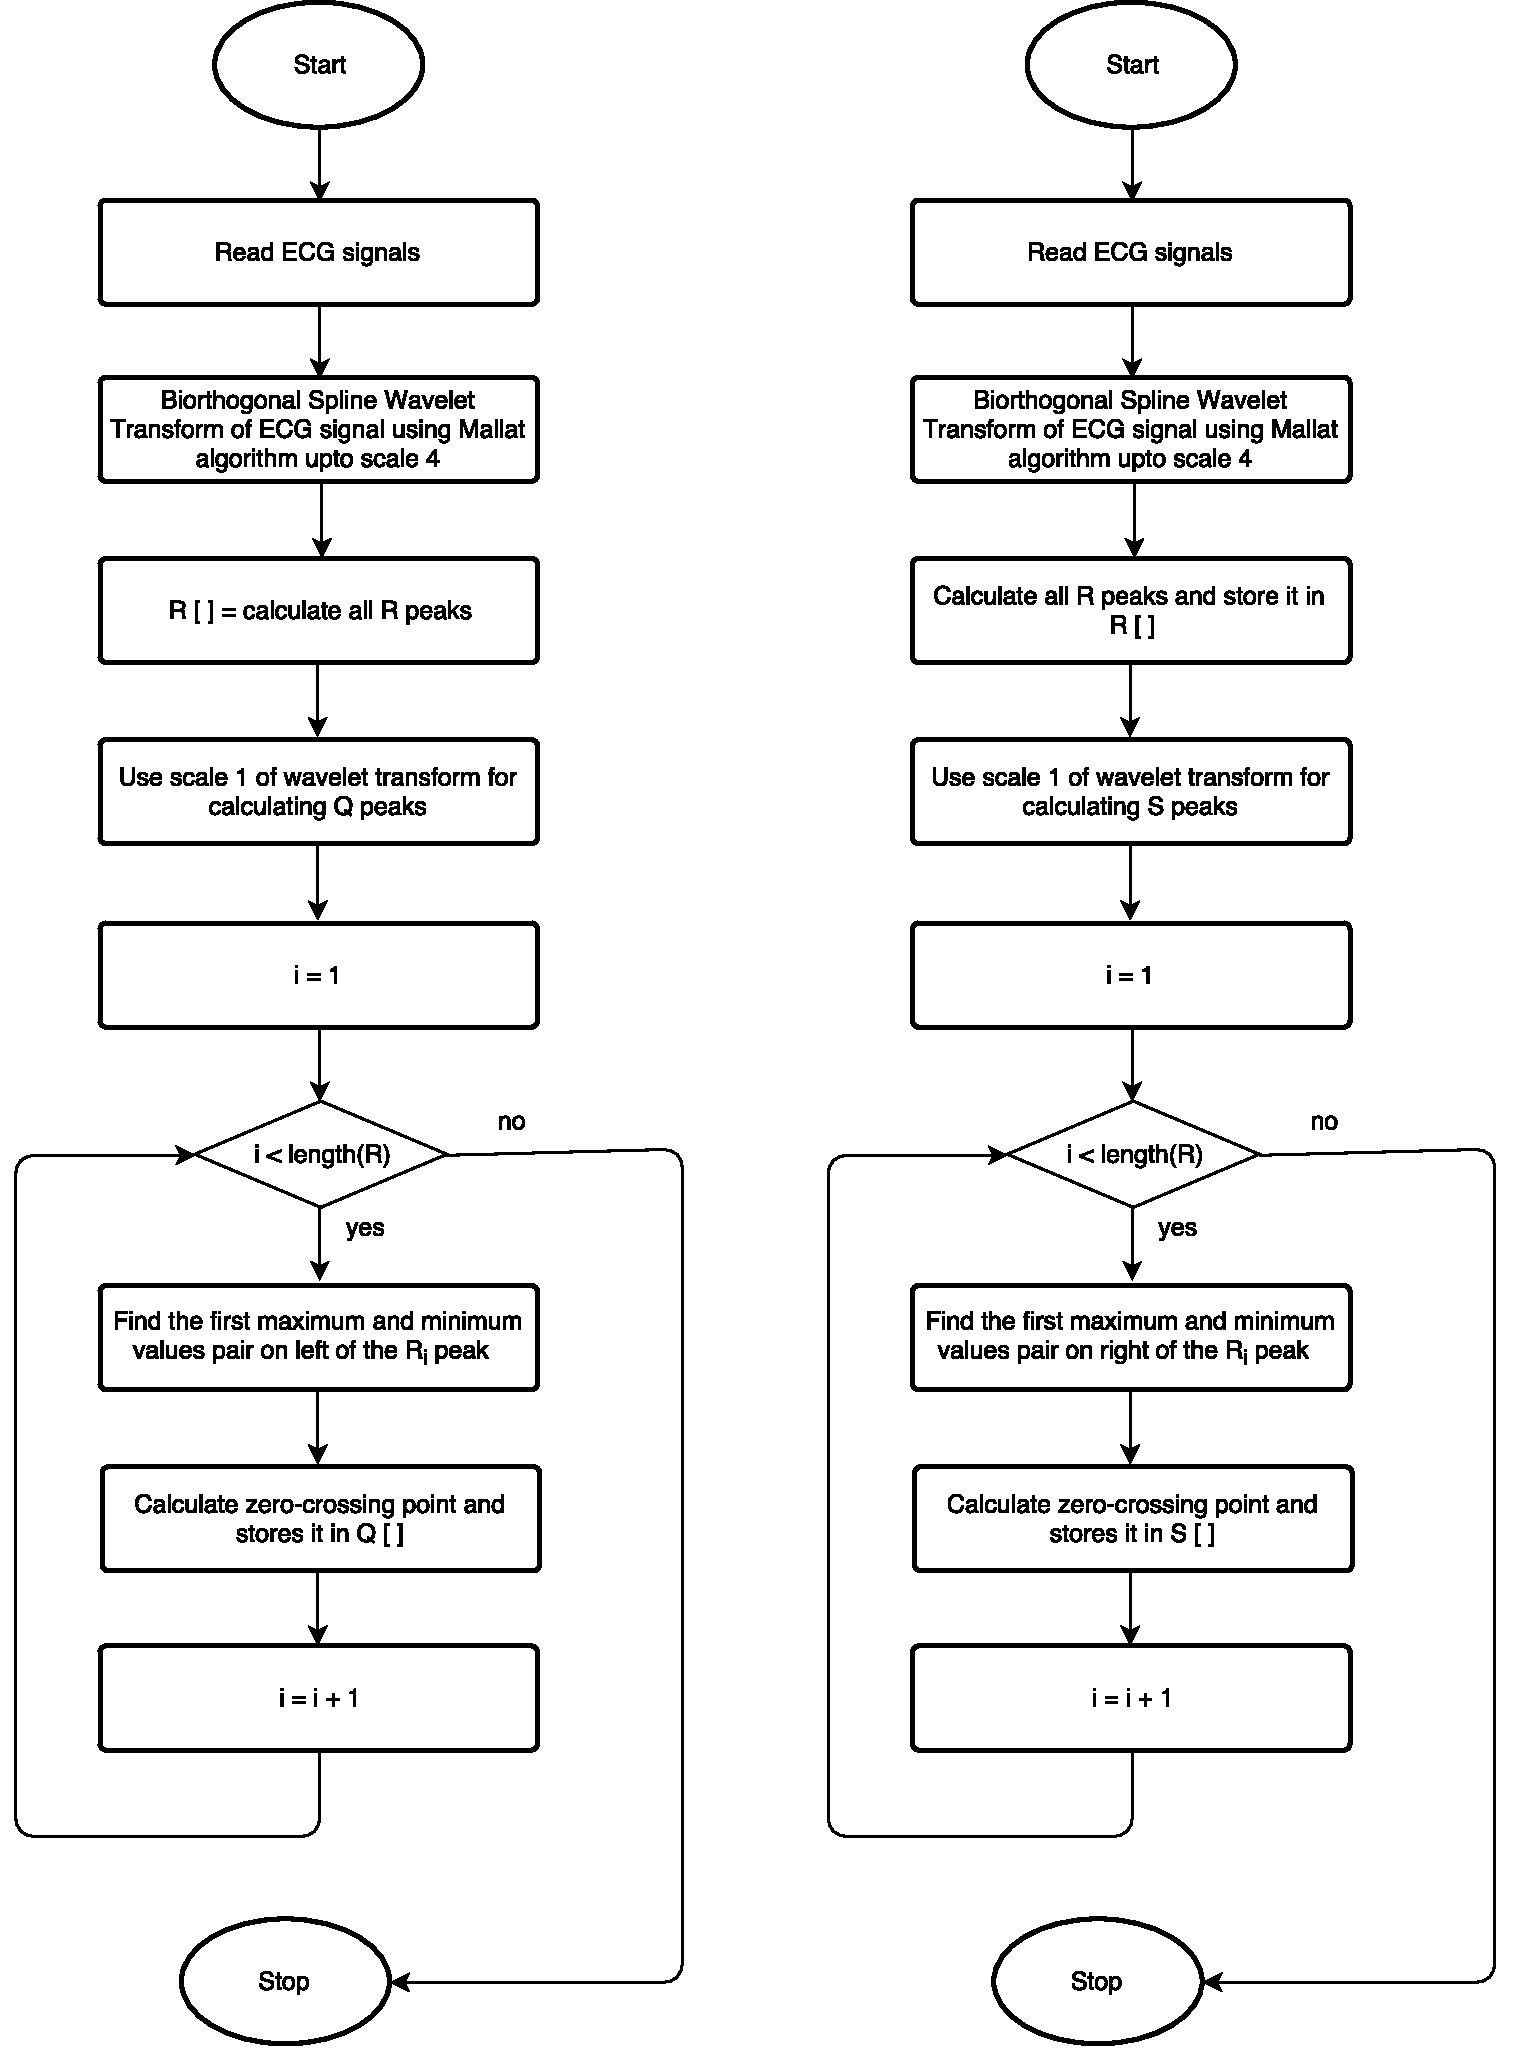
\includegraphics[width=25cm,height=22cm,keepaspectratio=true]{images/q-and-s.pdf}
	\caption{
		Flowchart for locating Q and S peaks.
	}
	\label{fig:qs}
\end{figure}

\bigskip

Q and S peaks generally are of high frequency. Therefore, their energies mainly lie at the $1^{st}$ scale. For finding the Q wave, the algorithm starts by looking on the left side of the R wave and finds the first non-zero value i.e. the Q wave. And because of the delay, the minimum value is searched in the window of 10 points to the detected Q wave. The same process is executed for the S wave, but in this case, the direction was on the right side of the R wave. The detected QRS complex can be seen in Figure \ref{fig:qrs_peaks}.

\begin{figure}[htpb]
	\centering
	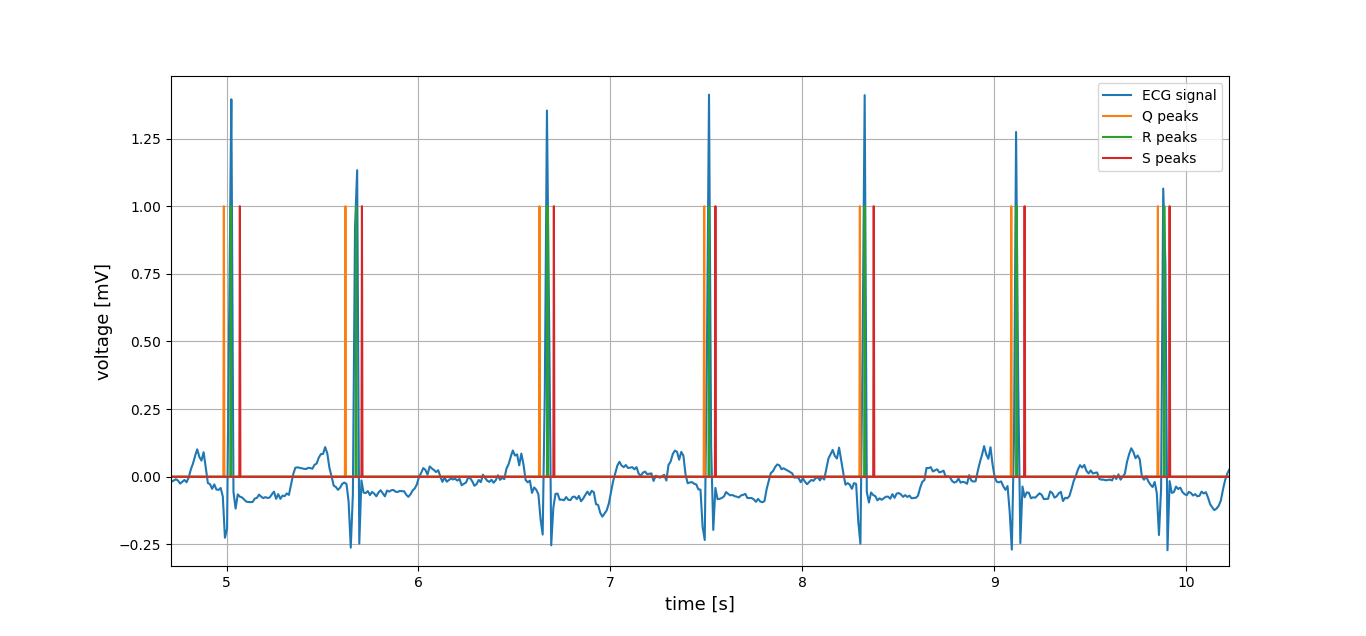
\includegraphics[width=15cm,height=15cm,keepaspectratio=true]{images/qrs}
	\caption{
		Detected Q, R and S peaks.
	}
	\label{fig:qrs_peaks}
\end{figure}







After detecting the QRS complex, P and T waves are required to be detected as they are important for the identification of the arrhythmia. P wave occurred before the QRS complex and T wave after the QRS complex. Therefore, they can be detected based on the QRS location.

\section{P and T Wave Detection}

After the detection of QRS complex, the P and T waves are also detected. According to power spectra of ECG signal \cite{4121752} and Table \ref{tab:qrsenergy}, most of the P and T waves energy lies at scale 4. Therefore, the scale 4 is selected to detect P and T waves. 

The corresponding modulus maxima pair of P and T waves can be seen in Figure \ref{fig:detail_coefficients} at scale 4 before and after the QRS complex. Therefore, P and T waves can be searched in a window before and after the QRS complex.
A window size of 100 is used for detecting the P wave and T waves. The P wave is searched within the 33\% of the average RR interval to the left of QRS complex and T wave is searched within the 67\% to the right of QRS complex. The P and T waves lie at the zero-crossing point of the identified modulus maxima pair in their respective windows. Because of the delay, a maximum value is searched in the window of 20 points to the zero-crossing point to determine the accurate position of P and T waves.

All detected waves are shown in Figure \ref{fig:pqrst}. The Flowchart for finding the P and T waves are shown in Figures \ref{fig:p_peaks_flow_chart} and \ref{fig:t_peaks_flow_chart} respectively.


\begin{figure}[htpb]
	\centering
	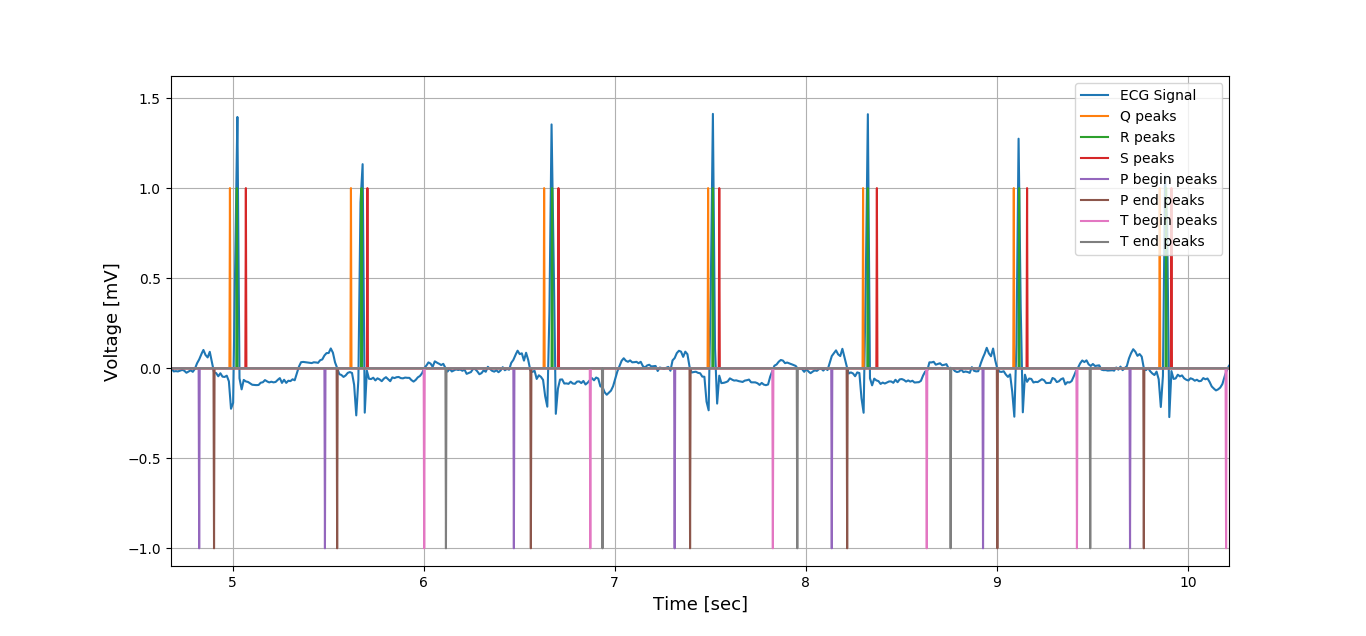
\includegraphics[width=15cm,height=15cm,keepaspectratio=true]{images/pqrst}
	\caption{
		Detected P,Q,R,S and T waves.
	}
	\label{fig:pqrst}
\end{figure}


\begin{figure}[htpb]
	\centering
	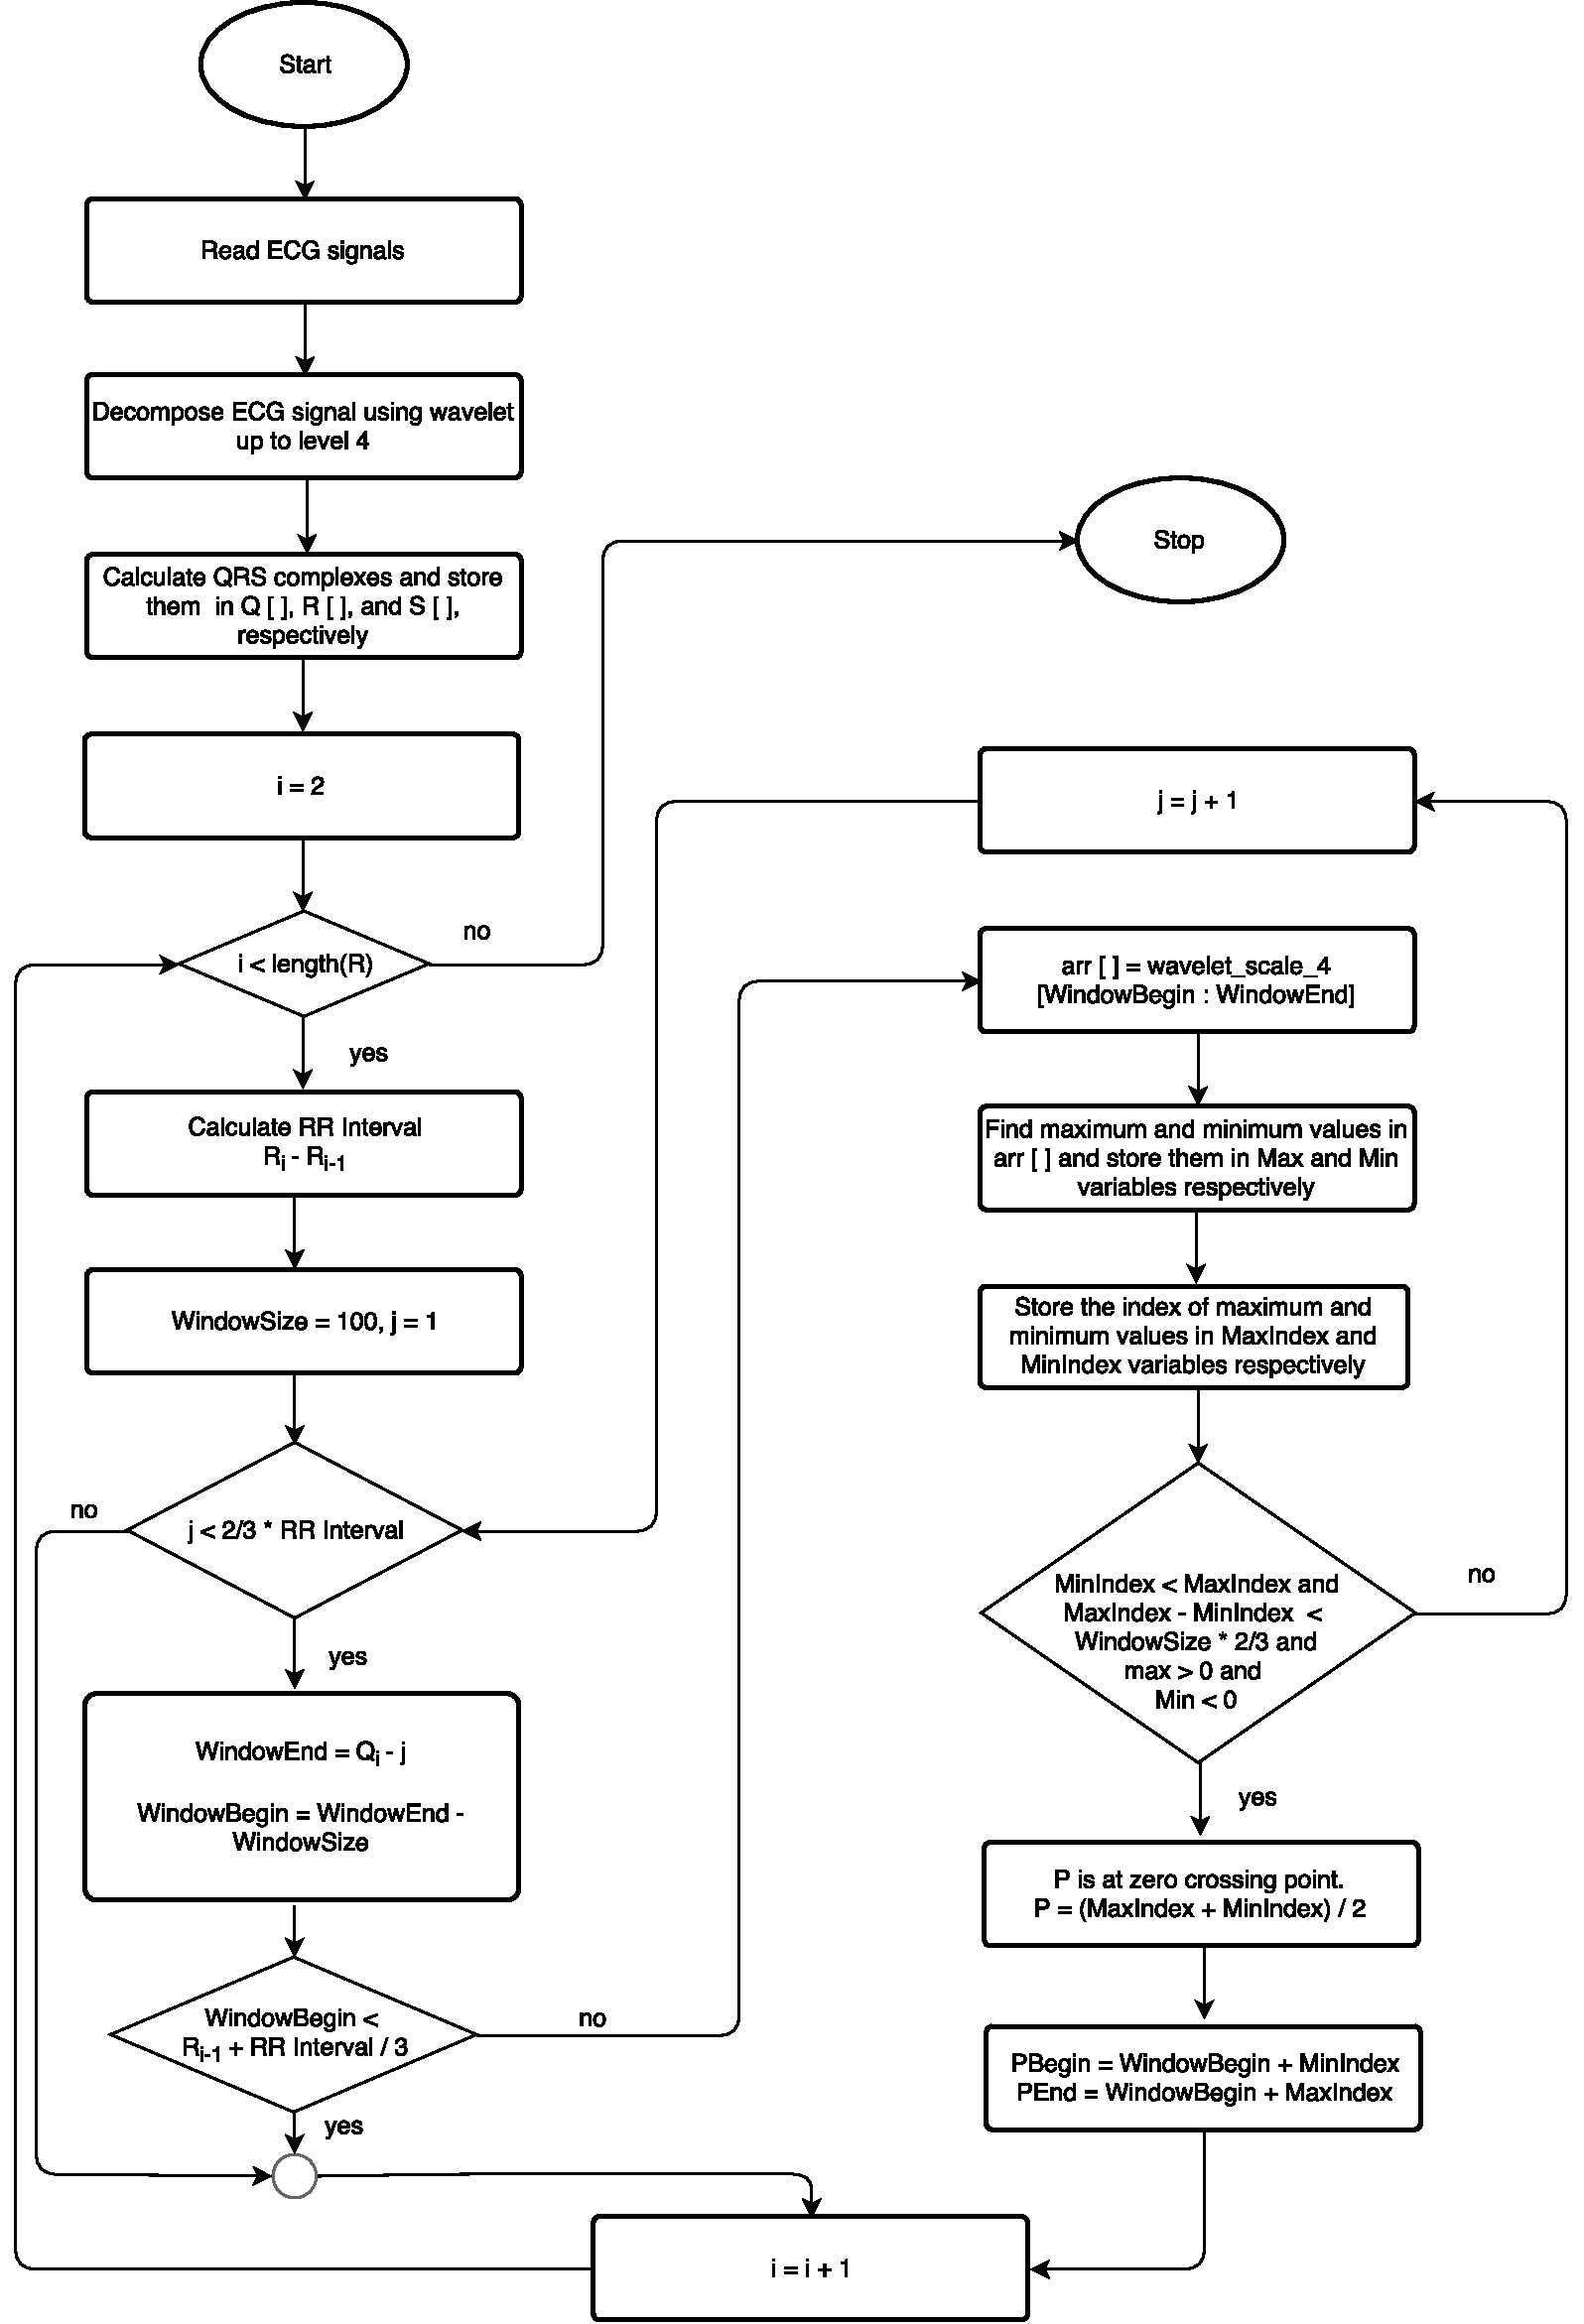
\includegraphics[width=25cm,height=22cm,keepaspectratio=true]{images/p_Wave.pdf}
	\caption{
		Flowchart for locating P wave.
	}
	\label{fig:p_peaks_flow_chart}
\end{figure}

\begin{figure}[htpb]
	\centering
	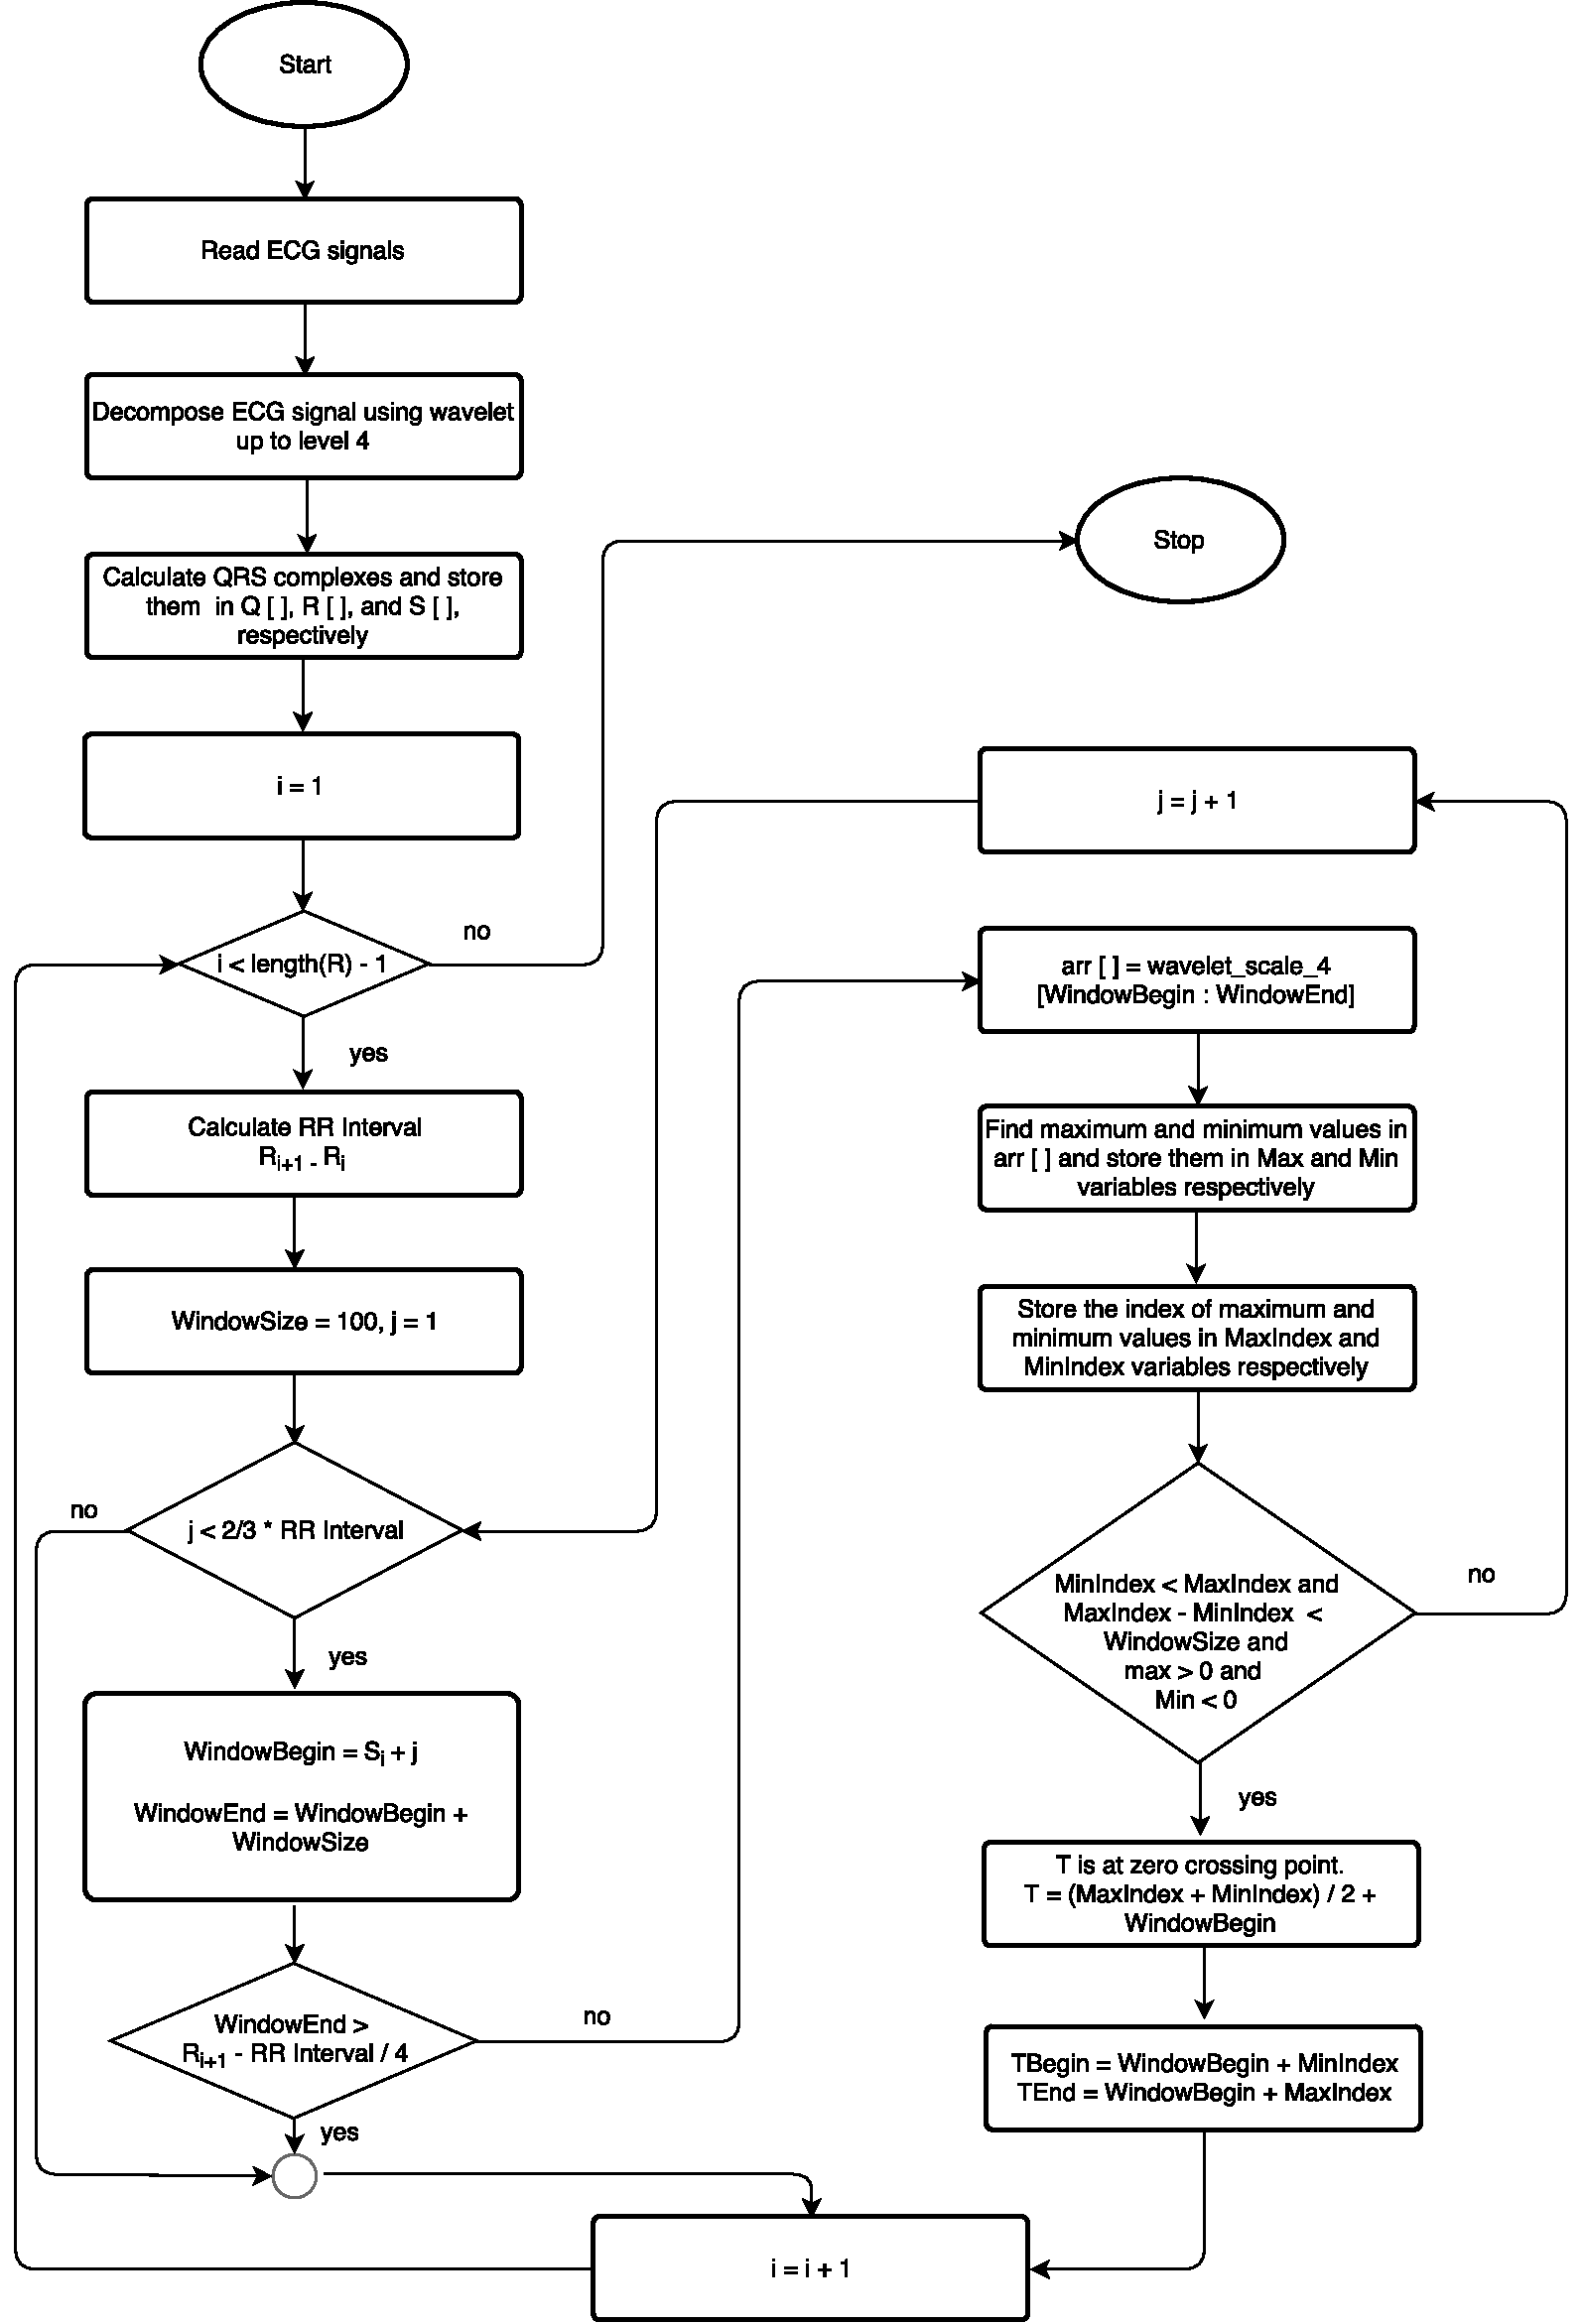
\includegraphics[width=25cm,height=22cm,keepaspectratio=true]{images/T_Wave.pdf}
	\caption{
		Flowchart for locating T wave.
	}
	\label{fig:t_peaks_flow_chart}
\end{figure}


\section{Heart Rate Calculation} \label{sec:heartrate}
The heart rate is calculated by using the RR interval. The formula to calculate the heart rate is:


\begin{equation}\label{eqn:heart_rate} 
HeartRate = sample\_rate \times \frac{60}{RR interval}
\end{equation}

where $sample\_rate$ is the sample rate of the ECG signal and 60 is multiplied to convert the heart rate into beats per minute.

\pagebreak

\section{Algorithm Execution on ECG Chair Data}
The data used in the development of ECG feature extraction algorithm is taken from MIT-BIH dataset and the algorithm works great with that dataset. The original ECG signal from the chair is shown in Figure \ref{fig:device_ecg_orignal} and the extracted features are shown in Figure \ref{fig:device_ecg_feature_extraction}.

\begin{figure}[htpb]
	\centering
	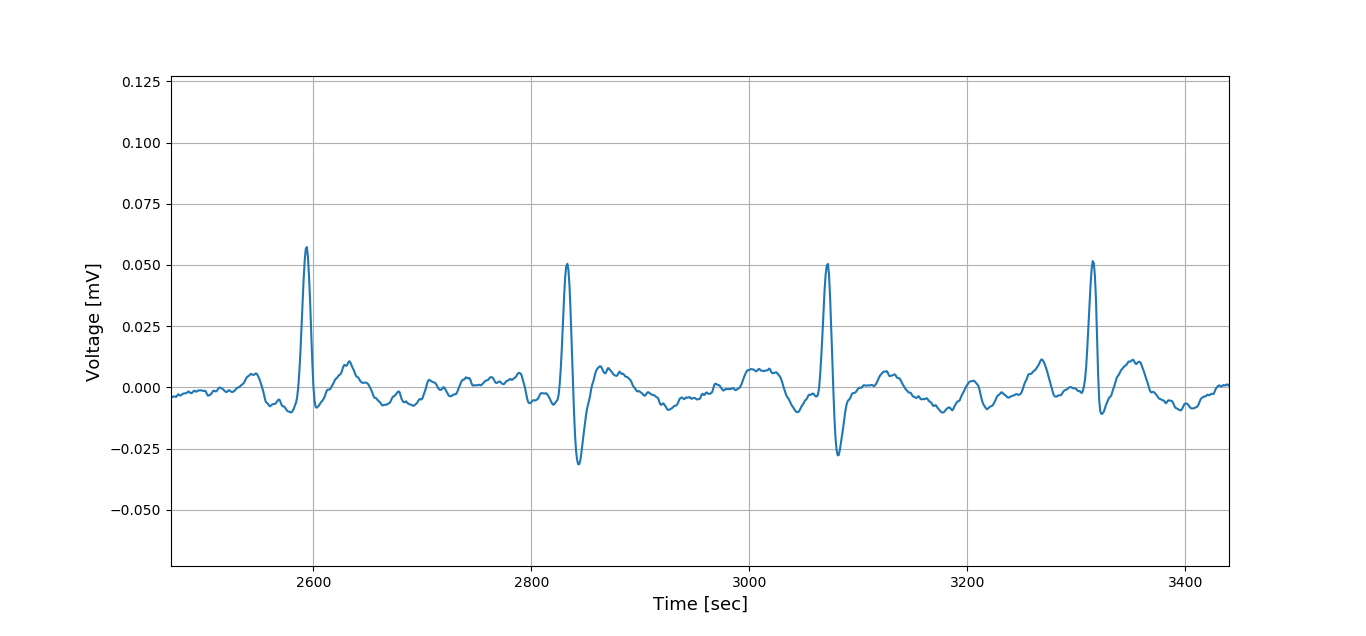
\includegraphics[width=15cm,height=15cm,keepaspectratio=true]{images/device_ecg_orignal}
	\caption{
		Original ECG signal from the chair.
	}
	\label{fig:device_ecg_orignal}
\end{figure}

\begin{figure}[htpb]
	\centering
	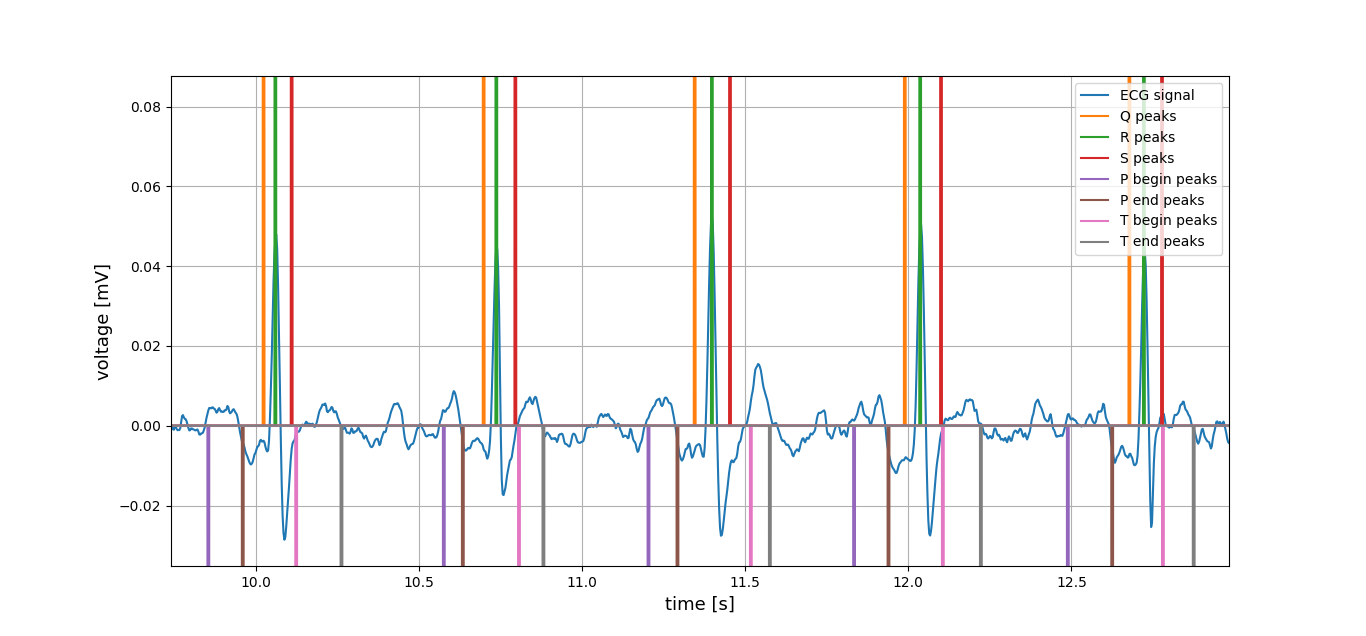
\includegraphics[width=15cm,height=15cm,keepaspectratio=true]{images/device_ecg_feature_extraction.png}
	\caption{
		Detected P,Q,R,S and T waves on the chair's ECG signal.
	}
	\label{fig:device_ecg_feature_extraction}
\end{figure}

\section{PPG Signal Processing}
A band-pass filter can be used to reduce the baseline drift and and high-frequency noise from the PPG signal. A passband of 0.5 Hz to 5 Hz has been used. After applying the band-pass filter, the resulting signal is the denoised PPG signal. The denoised channel 1 signal is shown in Figure \ref{fig:ppg_bandpass_denoised}. 

\begin{figure}[htpb]
	\centering
	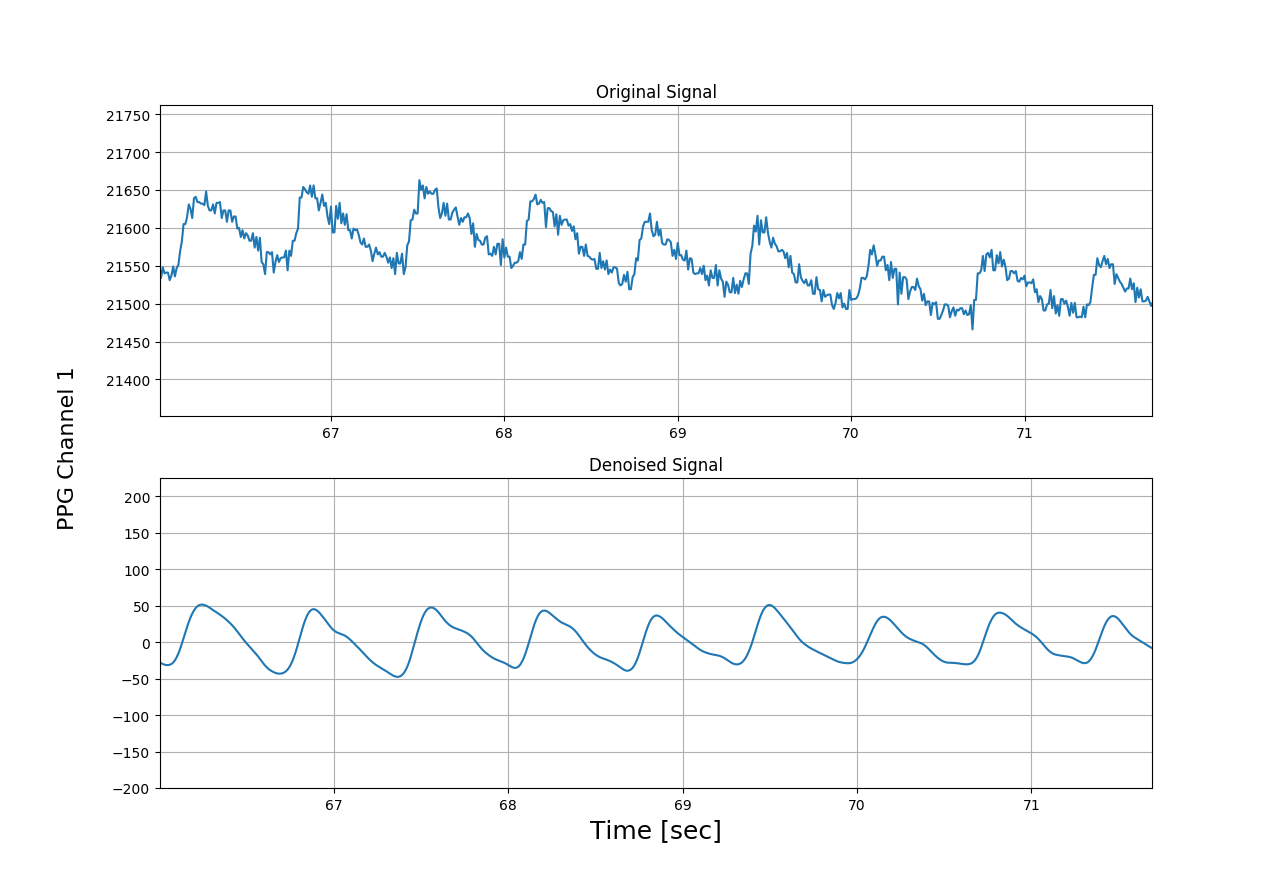
\includegraphics[width=15cm,height=15cm,keepaspectratio=true]{images/ppg_orig_denoised.png}
	\caption{
		The denoised PPG signal using band-pass filter.
	}
	\label{fig:ppg_bandpass_denoised}
\end{figure}